\chapter{Experimentation}
\label{ch:experimentation}
The theoretical analysis on Chapter \ref{ch:learning_augmented} provides the mathematical guarantees, but as previously stated, $Big$ $O$ Notation fails to capture the algorithms true efficiency gained from the machine learning aspect of \texttt{DIJKSTRA-PREDICTION}

This chapter therefore, presents a comprehensive experimental analysis and review of \texttt{DIJKSTRA-PREDICTION}, bench-marked against the classical \texttt{DIJKSTRA} algorithm, focusing entirely on the true reduction to the priority queue operations, resulting in an overall reduction in execution time.

More specifically, our experimental setup aims to evaluate:
\begin{itemize}
    \item The direct trade-off between the machine learning technique and the classical approach.
    \item The behavior of the Reserve Set ($R$) and thhe frequency on which the \texttt{UPDATE-PREDICTION} routine executes.
    \item The performance gain/loss between different oracle architectures, such as different neural (Multi-Layer Perceptrons) and gradient boosting models (XGBoost).
\end{itemize}

Our experiments are performed across tens of thousands of randomly generated graphs to ensure our evaluations are unbiased.
\newpage

\section{Dataset and Trace Extraction}
\label{sec:dataset}
Real-life networks, such as city road networks, are often inherently biased, for example with grid-like structures. To combat this issue, inorder to properly train and evaluate our machine learning oracle, we utilized the Erdős-Rényi\cite{erdos1960evolution} $G(n, p)$ random graph model to construct unbiased experimental scenarios, similar to Feijen and Schäfer\cite{feijenDijkstrasAlgorithmPredictions2023}. 


\subsection{Random Graph Generation (Erdős-Rényi)}
\label{subsec:erdos_renyi}

A custom Python data pipeline (\texttt{generate\_random\_graphs.py}) was developed to construct thousands of random topologies. Each generated graph $G=(V,E)$ is build according to the following rules:
\begin{itemize}
    \item \textbf{Vertices ($n$):} Each graph consists of precisely $n = 1000$ nodes.
    \item \textbf{Edge Probability ($p$):} To simulate realistic network sparsity, the expected out-degree of each node was set to $c = 8$. The probability of a directed edge existing between any two nodes is defined as $p = c / n = 0.008$.
    \item \textbf{Edge Weights ($w$):} To guarantee compliance with \textsc{DIJKSTRA}'s non-negative constraint, the weight $w(u,v)$ of every generated edge is drawn from a uniform random distribution between $(0, 1)$.
    \item \textbf{Target Nodes ($T$):} The expected number of target nodes per graph was set to $f = 20$. Each node is independently assigned as a target with probability $q = f / n = 0.02$. A fallback mechanism ensures that at least one valid target exists in $T$ if the pipeline results in an empty set.
\end{itemize}

The logic for generating these graphs is given in Algorithm \ref{alg:erdos}.

\begin{algorithm}[H]
\label{alg:erdos}
\caption{ERDOS-RENYI-GENERATOR ($n, c, f$)}
$p = c / n$, $q = f / n$\;
$V = \{0, 1, \dots, n-1\}$\;
$s = \text{RANDOM-INTEGER}(0, n-1)$\;
$T = \emptyset$, $E = \emptyset$\;

\tcp{Target Node Selection}
\For{$v \in V \setminus \{s\}$}{
    \If{$\text{RANDOM}() < q$}{
        $T \leftarrow T \cup \{v\}$\;
    }
}
\If{$T == \emptyset$}{
    $T \leftarrow \{\text{RANDOM-INTEGER}(0, n-1) \neq s\}$ \tcp*{Fallback}
}

\tcp{Edge Generation}
\For{$u \in V$}{
    $out\_degree \sim \mathcal{B}(n-1, p)$ \tcp*{Sample from binomial distribution}
    \If{$out\_degree > 0$}{
        $targets \leftarrow \text{RANDOM-SAMPLE}(V \setminus \{u\}, out\_degree)$\;
        \For{$v \in targets$}{
            $w \sim (0, 1)$ \tcp*{Sample from uniform distribution}
            $E \leftarrow E \cup \{(u, v, w)\}$\;
        }
    }
}
\Return $G=(V, E), s, T$
\end{algorithm}
\newpage

\subsection{Trace Extraction}
\label{subsec:trace_extraction}
In order to train our machine learning networks we require a supervised learning dataset. To achieve this each graph in our dataset must be converted into a feature vector $X$ (the algorithmic $trace$)\footnote{Explanation for the structure of the $trace$ was given in Section \ref{sec:prinicples}} and a corresponding label $y$ (the true shortest path).

For every generated graph, a \texttt{DIJKSTRA} execution is initiated from a randomly selected source node $s$. The algorithm executes exactly $i_0 = 10$ steps. At each step $i \in \{1, 2, \dots, i_0\}$, the system records two values:

\begin{enumerate}
    \item $d_i$: The distance of the node currently extracted from the priority queue (representing the expanding lower bound).
    \item $B_i$: The current best-known upper bound to any target $t \in T$. If no target has been discovered yet, this is represented as $0.0$ for the model (to avoid \texttt{Infinity} errors).
\end{enumerate}


When this process finalizes, it returns a 20-dimensional feature vector array $X = [d_1, B_1, d_2, B_2, \dots, d_{10}, B_{10}]$. After the initial $i_0$ steps, the algorithm resumes execution until it settles the first target node, recording the true shortest path distance $D$. This value is the target label $y$ for our supervised learning models.

If the algorithm happens to find target $t \in T$ in the first $i_0$ steps, then the graph is discarded from the training set, as it contains less than the required 20 features.

Through this pipeline, we generated a total of 80,000 valid graphs for the training of the models. For each graph, their corresponding $trace$ was then compiled into a final unified CSV dataset, ready to be used. 

The execution mechanics for extracting the supervised feature vector $X$ and the label $y$ from any given graph are detailed in Algorithm \ref{alg:trace_extract}.


\begin{algorithm}[htbp]
\caption{TRACE-EXTRACTOR ($G, s, T, i_0$)}
\label{alg:trace_extract}
$d(v) = \infty$ \textbf{for all} $v \in V$, $d(s) = 0$\;
PQ.INSERT$(s, 0)$\;
$B = \infty$, $X = \emptyset$, $y = \text{NULL}$\;
$i = 0$, $S = \emptyset$ \tcp*{Settled nodes}

\While{\textbf{not} PQ.EMPTY()}{
    $u = \text{PQ.REMOVE-MIN}()$\;
    \If{$u \in S$}{\textbf{continue}}
    
    $S \leftarrow S \cup \{u\}$\;
    $i = i + 1$\;
    
    \If{$i \le i_0$}{
        \eIf{$B == \infty$}{
            $B_{formatted} = 0.0$\;
        }{
            $B_{formatted} = B$\;
        }
        $X \leftarrow X \cup \{d(u), B_{formatted}\}$ \tcp*{Append to feature vector}
    }
    
    \If{$u \in T$}{
        $y = d(u)$ \tcp*{Optimal shortest path found}
        \textbf{break}\;
    }
    
    \For{$(u,v) \in E$}{
        \If{$v \in S$}{\textbf{continue}}
        $tent = d(u) + w(u,v)$\;
        \If{$v \in T$}{
            $B = \min(B, tent)$\;
        }
        \If{$tent < d(v)$}{
            $d(v) = tent$\;
            PQ.INSERT$(v, tent)$\;
        }
    }
}

\If{$y == \text{NULL}$ \textbf{or} $i \le i_0$}{
    \Return \text{INVALID} \tcp*{Graph is invalid for training}
}
\Return $X, y$
\end{algorithm}

\section{Oracle Architecture and Model Training}
\label{sec:oracle_training}

With the generation of the 80,000 algorithmic traces and their optimal shortest path distances, the problem is structured as a supervised regression task. The objective is to train a machine learning oracle capable of accurately mapping the $i_0$-step algorithmic trace $X$ to the predicted target distance $P$. 

The dataset was split into a training set (80\%) and a testing set (20\%), for evaluation purposes before the final benchmark test. To guarantee proper experimental tracking, all hyperparameter configurations and resulting metrics were tracked utilizing the \texttt{MLflow} platform.  

We evaluate two machine learning models for the role of the prediction oracle: Multi-Layer Perceptrons (MLP)\cite{rumelhartLearningRepresentationsBackpropagating1986} and Gradient Boosting Decision Trees (XGBoost)\cite{chenXGBoostScalableTree2016}.


\subsection{Multi-Layer Perceptron (MLP) Configurations}
\label{subsec:mlp_training}

Similar to Feijen and Schäfer we utilized the \texttt{MLPRegressor}. The models were configured to train for a maximum of 1000 iterations (\texttt{max\_iter}). 

We tested five different hidden-layer architectures, utilizing two hidden layers of varying widths: $(8, 8)$, $(16, 16)$, $(32, 32)$, $(64, 64)$, and $(128, 128)$.

\begin{figure}[htbp]
    \centering
    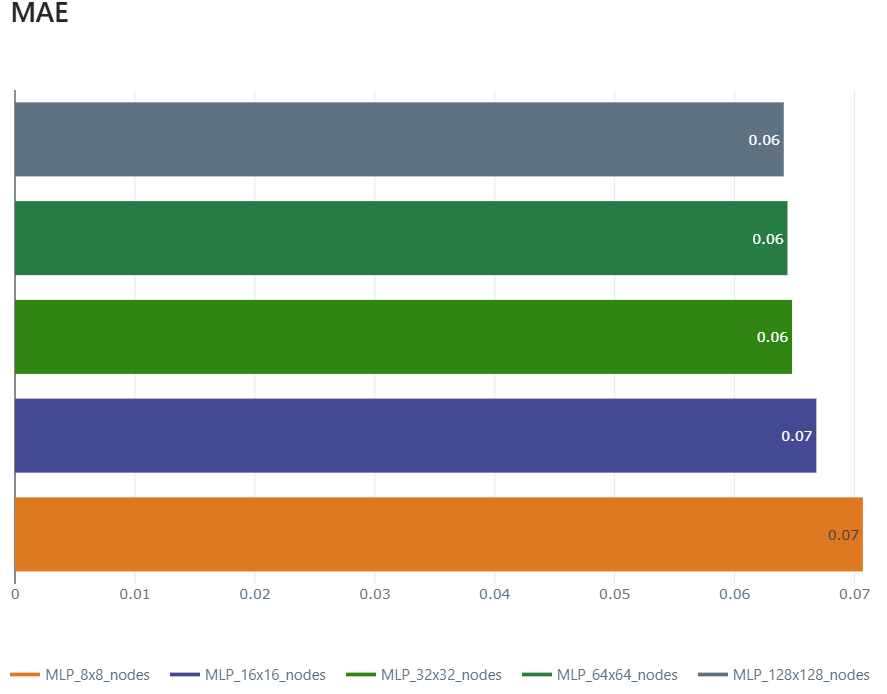
\includegraphics[width=0.8\linewidth]{tex/images/mlp_mae.png}
    \caption{Mean Absolute Error (MAE) evaluation of various MLP architectures}
    \label{fig:mlp_mae}
    
    \vspace{0.5cm} % Προσθέτει λίγο κενό ανάμεσα στις δύο εικόνες
    
    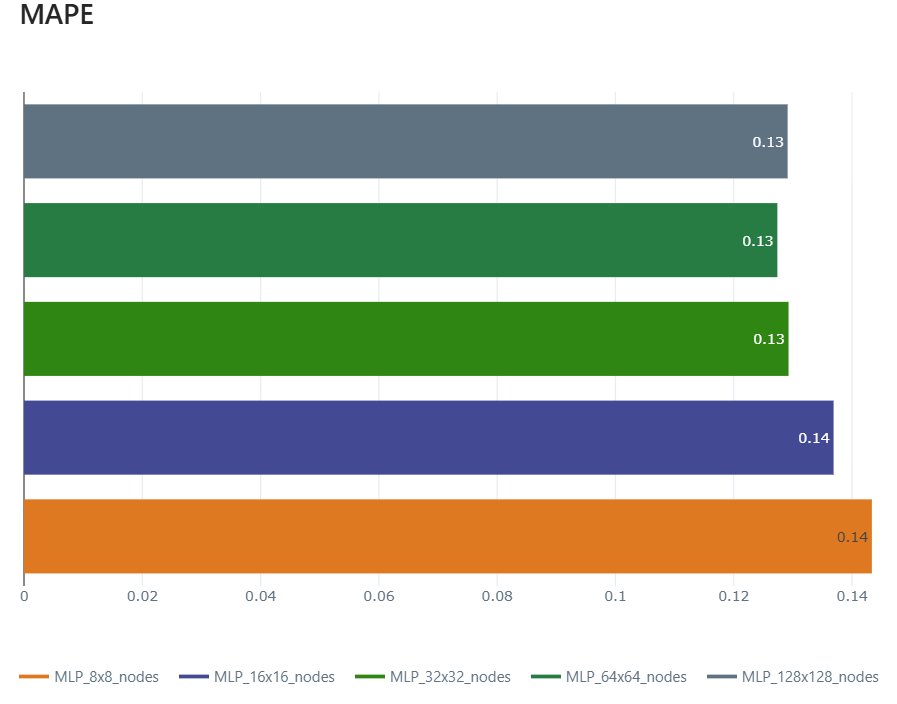
\includegraphics[width=0.8\linewidth]{tex/images/mlp_mape.png}
    \caption{Mean Absolute Percentage Error (MAPE) evaluation of various MLP architectures}
    \label{fig:mlp_mape}
\end{figure}
\newpage


\begin{table}[h]
\centering
\caption{Performance metrics of various MLP architectures.}
\label{tab:mlp_metrics}
\renewcommand{\tabularxcolumn}[1]{m{#1}}
\begin{tabularx}{\textwidth}{
    >{\centering\arraybackslash}X 
    >{\centering\arraybackslash}X 
    >{\centering\arraybackslash}X
}
\toprule
\textbf{Model Architecture} & \textbf{Mean Absolute Error (MAE)} & \textbf{Mean Absolute Percentage Error (MAPE)} \\ \midrule
128x128 & 0.0641008 & 0.12911040 \\
64x64   & 0.0644093 & 0.12737545 \\
32x32   & 0.0647925 & 0.12926555 \\
16x16   & 0.0668187 & 0.13688045 \\
8x8     & 0.0706973 & 0.14335474 \\ \bottomrule
\end{tabularx}
\end{table}


According to the training results (see Figures \ref{fig:mlp_mae} and \ref{fig:mlp_mape} and Table \ref{tab:mlp_metrics}), scaling the model's architecture provides an improvement, especially in the beginning. The $(8, 8)$ architecture results in a \(\approx \)0.0706 MAE value and a \(\approx \)0.1433 MAPE value. The $(16, 16)$ architecture shows a notable improvement with a \(\approx \)0.0668 MAE value and a \(\approx \)0.1368 MAPE value. Further scaling the model to a $(32, 32)$ architecture shows a drop into a  \(\approx \)0.0647 MAE value and a  \(\approx \)0.1292 MAPE value, but notably, continuing to scale the architecture into $(64, 64)$, and $(128, 128)$ yields no measurable improvement in either metric, introducing the law of diminishing returns.

Since the oracle model executes synchronously within the loop of the \texttt{DIJKSTRA-PREDICTION} algorithm, we require our model to be lightweight, so as to not incur heavy computational loads leading to an overall worse performance in time execution compared to \texttt{DIJKSTRA}. Notably for our interactive environment, we deployed an MLP architecture of $(16, 16)$ following Feijen's and Schäfer's chosen oracle.

\subsection{Gradient Boosting (XGBoost) Variants}
\label{subsec:xgboost_training}

While Feijen and Schäfer deployed an MLP to act as an oracle, for our experiments we consider the alternative use of a tree ensemble method. XGBoost often achieves superior performance and faster inference time on tabular data.

We trained three XGBoost architectures. For the purposes of this thesis we denote an XGBoost configuration as $\text{XGBoost}(n, d, \eta)$ where $n$ is the number of estimators, $d$ is the maximum depth, and $\eta$ is the learning rate:

\begin{itemize}
    \item \textbf{XGBoost Fast (100, 3, 0.1):} Configured with 100 estimators, a maximum tree depth of 3, and a learning rate of 0.1. This variant is designed for fast inference, minimizing the time reduction taken for the prediction of the value P.
    \item \textbf{XGBoost Medium (200, 4, 0.05):} Configured with 200 estimators, a maximum tree depth of 4, and a learning rate of 0.05. This variant was designed as a middle ground.
    \item \textbf{XGBoost Deep (300, 5, 0.05):} Configured with 300 estimators, a maximum tree depth of 5, and a learning rate of 0.05. This variant is designed to minimize the error of the prediction.
\end{itemize}

\begin{table}[h]
\centering
\caption{Performance metrics of the evaluated XGBoost architectures.}
\label{tab:xgboost_metrics}
\renewcommand{\tabularxcolumn}[1]{m{#1}}
\begin{tabularx}{\textwidth}{
    >{\centering\arraybackslash}X 
    >{\centering\arraybackslash}X 
    >{\centering\arraybackslash}X
}
\toprule
\textbf{Model Architecture} & \textbf{Mean Absolute Error (MAE)} & \textbf{Mean Absolute Percentage Error (MAPE)} \\ \midrule
XGBoost Deep (300,5,0.05)  & 0.0637316 & 0.1271240 \\
XGBoost Medium (200,4,0.05) & 0.0651171 & 0.1303728 \\
XGBoost Fast (100,3,0.1)  & 0.0669162 & 0.1345042 \\ \bottomrule
\end{tabularx}
\end{table}


\begin{figure}[htbp]
    \centering
    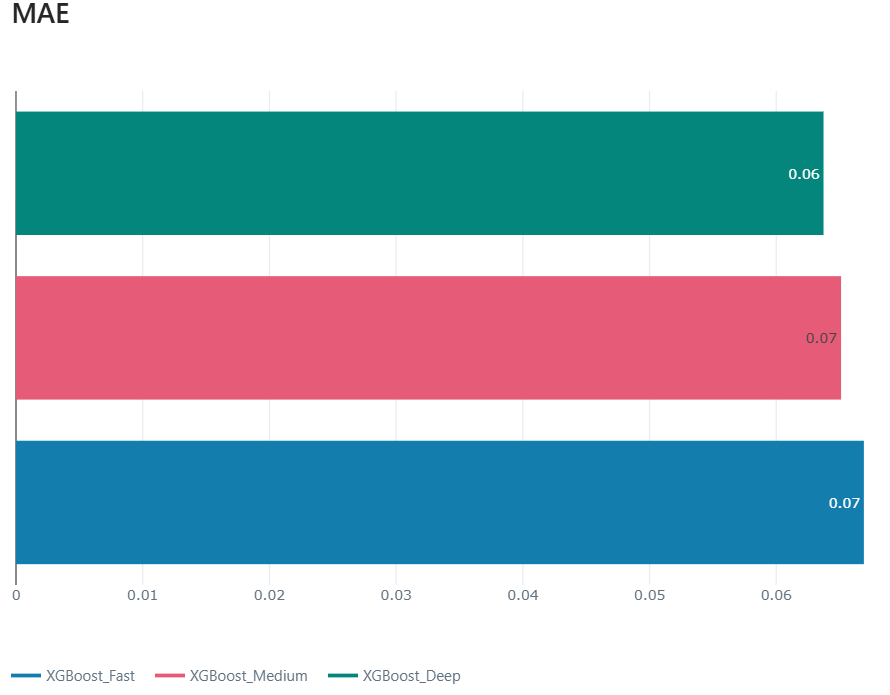
\includegraphics[width=0.8\linewidth]{tex/images/xgboost_mae.png}
    \caption{Mean Absolute Error (MAE) evaluation of XGBoost variants}
    \label{fig:xgboost_mae}
    
    \vspace{0.5cm} 
    
    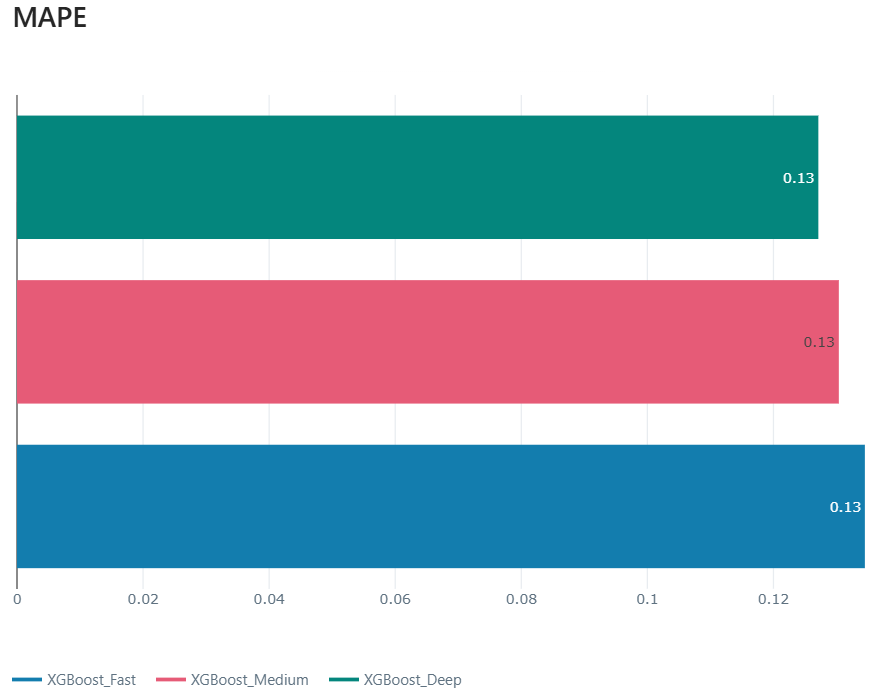
\includegraphics[width=0.8\linewidth]{tex/images/xgboost_mape.png}
    \caption{Mean Absolute Percentage Error (MAPE) evaluation of XGBoost variants.}
    \label{fig:xgboost_mape}
\end{figure}
\newpage

According to the training results (See Figure \ref{fig:xgboost_mae} and \ref{fig:xgboost_mape}, and Table \ref{tab:xgboost_metrics}) the gradient boosting approach demonstrates a similar performance to the MLP approach. XGBoost Fast (100,3,0.1) achieved a \(\approx \)0.0669 MAE value and a \(\approx \)0.1345 MAPE value. XGBoost Medium (200,4,0.05) performed slightly better with a \(\approx \)0.0651 MAE value and a \(\approx \)0.1303 MAPE value. Finally, XGBoost Deep (300,5,0.05) performed overall better, with a \(\approx \)0.0637 MAE value and a \(\approx \)0.1271 MAPE value.
Similarly to the MLP deployment, we require the XGBoost model used to be lightweight. 

Despite the performance of the XGBoost models there is a fundamental flaw making them unviable for predictions outside the Erdős-Rényi graph generation model. Decision tree models are notoriously \textit{bad} at extrapolation. In other words, because decision trees partition the feature space into regions and as a result they cannot predict values larger than the maximum target observed during the training phase. For example an XGBoost model trained on the Erdős-Rényi graph generation model ((0,1) weight distribution) would be unable to predict a correct value in our interactive enviroment if a user chose to assign weight weight ranging from 10 to 1000, since the final target value (the final total path distance) is likely to be several times larger than one encountered during training. 

In contrast, MLPs map inputs through mathematical weight transformations, allowing them to extrapolate values to unseen numerical ranges. Therefore, while XGBoost provides sufficient results in our local experiments, the MLP architecture chosen by Feijen and Schäfer remains the best option for a user-driven application.

Still, if trained on a dataset where the training maximum target values remain consistent and relevant in relation to a deployment environment, the extrapolation flaw becomes irrelevant, Therefore, we will still consider the gradient boosting approach in our following experiments. This enables us to evaluate the impact this approach can have on Priority Queue operations and finally overall execution time.
\newpage

\subsection{Evaluating Alternative Architectures}
\label{subsec:alternative_architectures}

Besides Multi-Layer Perceptrons and Gradient Boosting, one can consider using a state-of-the-art model such as Graph Neural Networks (GNNs)\cite{scarselliTheGraphNeuralNetworkModel2009} or Attention-based Transformers\cite{vaswaniAttentionAllYou2023}. These models are better suited for capturing graph topologies and long-range relationships and can predict a $P$ value with higher accuracy thus further reducing the priority queue operations in large scale graphs.

The issue with implementing such models arises when solving for the shortest overall execution time. The computational cost and memory required for their inference phase would be considerably larger compared to more lightweight methods such as MLP and XGBoost. This delay would result in a larger delay for the prediction of the oracle and would therefore render the \texttt{DIJKSTRA-PREDICTION} algorithm slower compared to \texttt{DIJKSTRA}. Consequently, we won't consider heavier models in our experiments.

\section{Comparative Results}
\label{sec:results}

The MAE and MAPE values evaluated in Section \ref{sec:oracle_training} provide insights into the model's accuracy. In order to compare \texttt{DIJKSTRA-PREDICTION} to \texttt{DIJKSTRA} we bench-marked the execution of the two algorithms against each other, utilizing the oracles presented. 

The test set consist of 10,000 generated graph, following the Erdős-Rényi graph generation model (See Section \ref{subsec:erdos_renyi}) with parameters ($n=1000, c=8, f=20$). \texttt{DIJKSTRA-PREDICTION} was set to make a prediction at $i_0 = 10$, and we defined $\alpha = 1.1$ and $\beta = 1.2$.

All resulting data were tracked utilizing the \texttt{MLflow} platform and were exported and visualized using the \texttt{Matplotlib} and \texttt{Seaborn} frameworks. 
\newpage

\subsection{Algorithmic Execution of MLP Oracle Architectures}
\label{subsec:mlp_benchmark}

We begin our evaluation by comparing for the MLP oracle model variants.

Table \ref{tab:mlp_prio} and Figures \ref{fig:mlp_prio} and \ref{fig:mlp_skipped_prio} showcase the average priority queue operations compared to \texttt{DIJKSTRA} and furthermore a comparison on average priority queue operations skipped by each oracle model.

\begin{table}[h]
\centering
\caption{Priority Queue Operations with MLP oracle architectures.}
\label{tab:mlp_prio}
\renewcommand{\tabularxcolumn}[1]{m{#1}}
\begin{tabularx}{\textwidth}{
    >{\centering\arraybackslash}X 
    >{\centering\arraybackslash}X 
    >{\centering\arraybackslash}X
}
\toprule
\textbf{Oracle Model Architecture} & \textbf{Average Priority Queue Operations} & \textbf{Average Priority Queue Operation Skips} \\ \midrule
MLP(128x128) & 139.18 & 243.50 \\
MLP(64x64)   & 138.74 & 243.95 \\
MLP(32x32)   & 138.71 & 243.98 \\
MLP(16x16)   & 139.44 & 243.25 \\
MLP(8x8)     & 138.87 & 243.82 \\ \midrule
\texttt{DIJKSTRA} & 382.7 & -  \\ \bottomrule
\end{tabularx}
\end{table}

\begin{figure}[h]
    \centering
    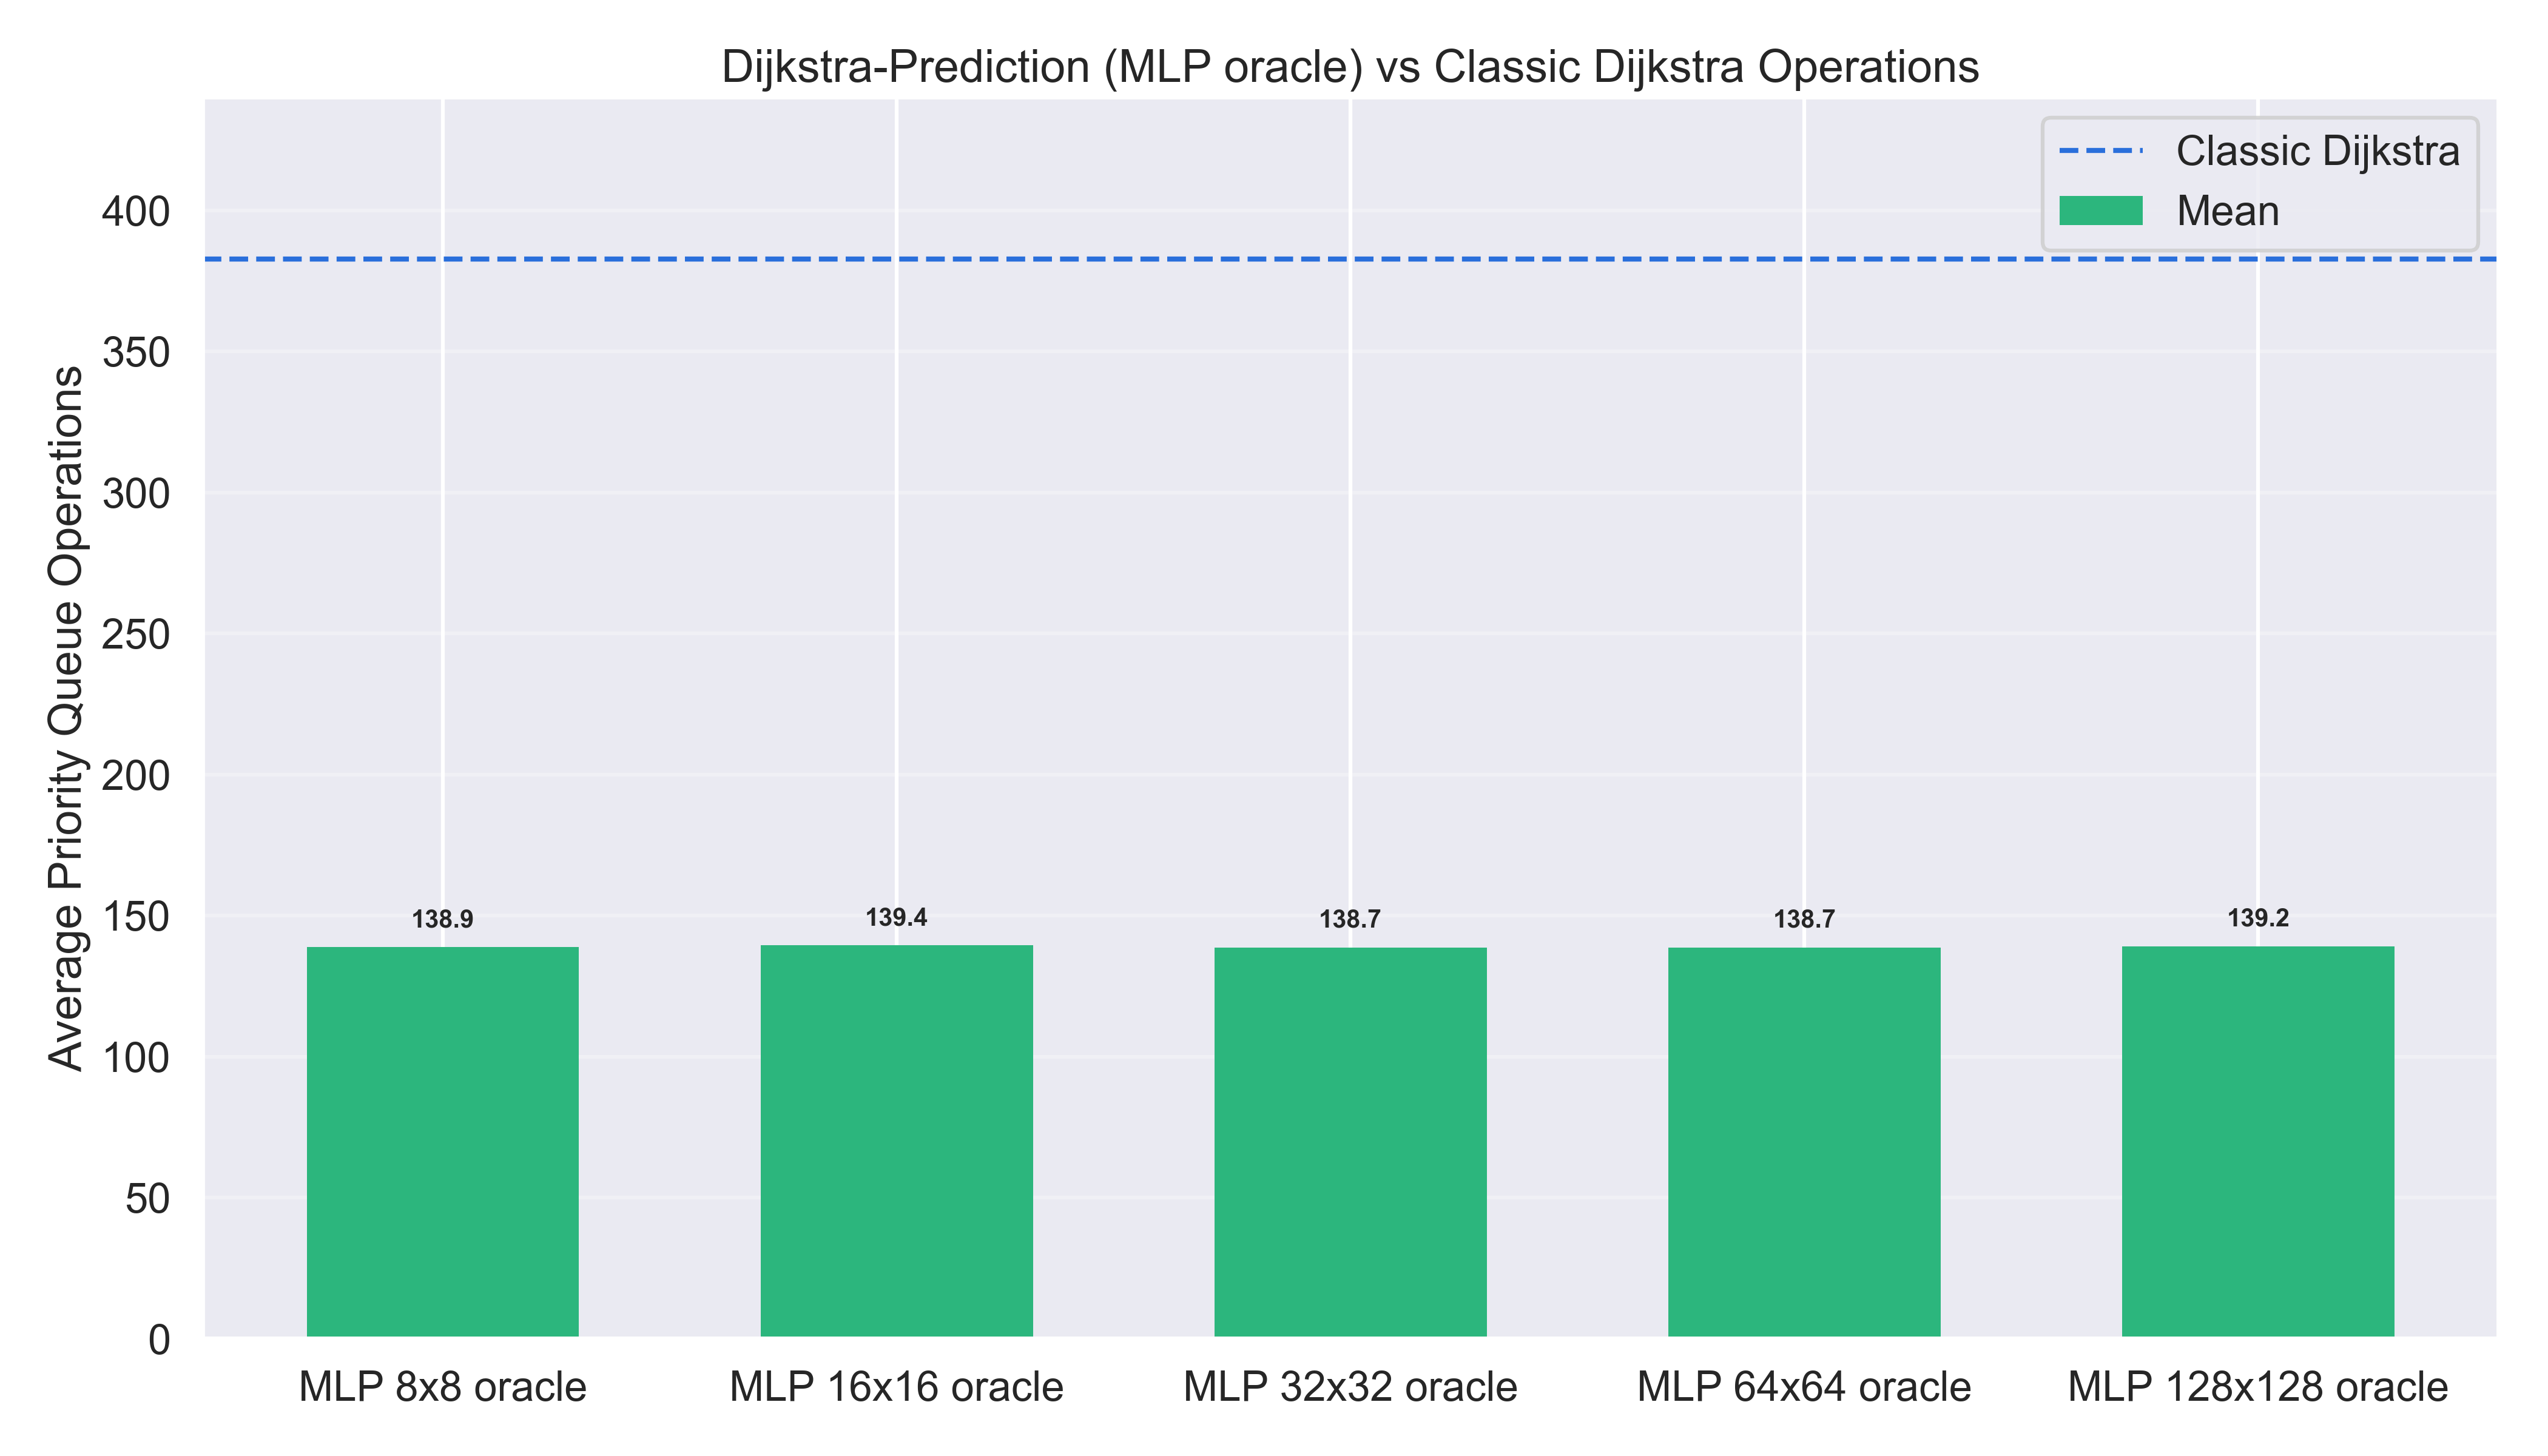
\includegraphics[width=1\linewidth]{tex/images/mlp_ops_comparison.png}
    \caption{Average operations achieved via prediction pruning (MLP).}
    \label{fig:mlp_prio}
\end{figure}

\begin{figure}[h]
    \centering
    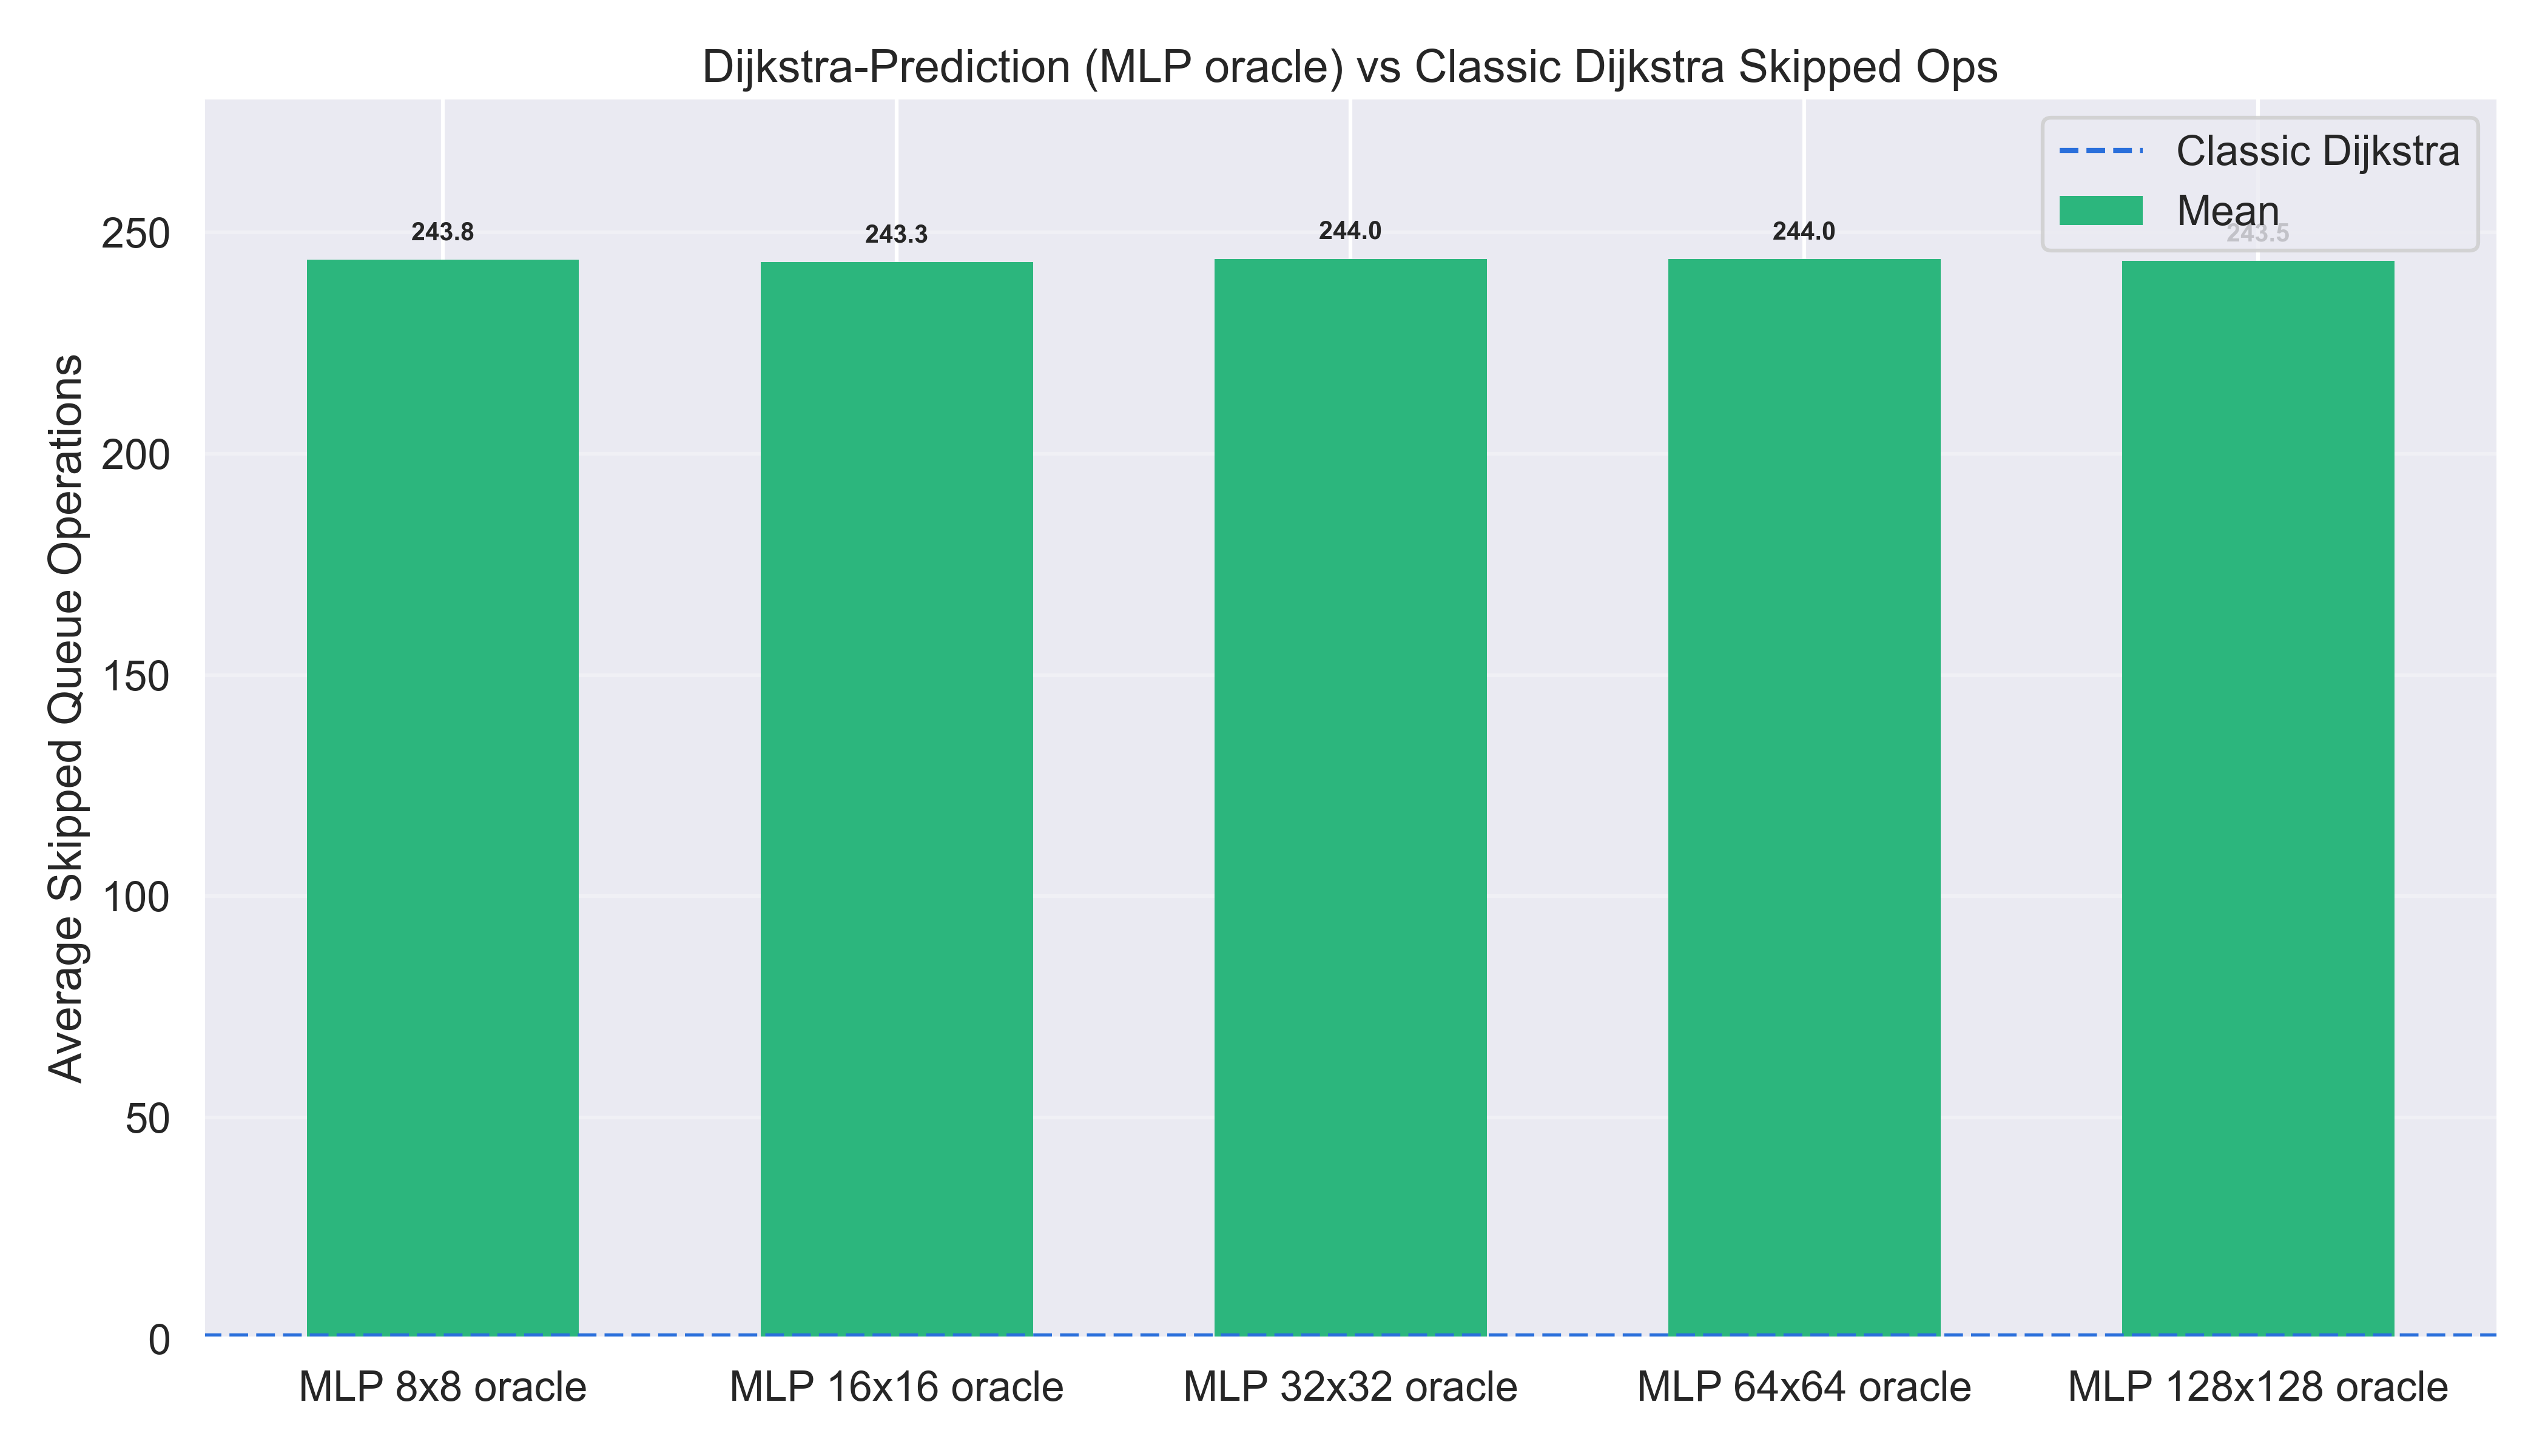
\includegraphics[width=1\linewidth]{tex/images/mlp_skipped_ops_comparison.png}
    \caption{Average skipped operations achieved via prediction pruning (MLP).}
    \label{fig:mlp_skipped_prio}
\end{figure}


The classic \texttt{DIJKSTRA} algorithm required an average of 382.7 operations per graph compared to \texttt{DIJKSTRA-PREDICTION} which showcased a significant reduction of more than 60\% leading to an average of $\approx 139$ operations per graph, skipping $\approx 243.5$ operations depending on the oracle model used.

It is important to note that scaling the neural network architecture provided no algorithmic benefit.

We also tracked the behavior of the Reserve Set ($R$). Table \ref{tab:mlp_reserve} and Figures \ref{fig:mlp_r_inserts} and \ref{fig:mlp_r_rescues} showcase the use of the Reserve Set ($R$), both in average reserve set inserts and average reserve set rescues, in order to evaluate its use through out the algorithm.

\begin{table}[h]
\centering
\caption{Reserve Set Operations with MLP oracle architectures.}
\label{tab:mlp_reserve}
\renewcommand{\tabularxcolumn}[1]{m{#1}}
\begin{tabularx}{\textwidth}{
    >{\centering\arraybackslash}X 
    >{\centering\arraybackslash}X 
    >{\centering\arraybackslash}X
}
\toprule
\textbf{Oracle Model Architecture} & \textbf{Average Reserve Set Inserts} & \textbf{Average Reserve Set Rescues} \\ \midrule
MLP(128x128) & 31.36 & 5.92 \\
MLP(64x64)   & 32.52 & 6.64 \\
MLP(32x32)   & 32.63 & 6.73 \\
MLP(16x16)   & 30.99 & 5.80 \\
MLP(8x8)     & 32.57 & 6.83 \\ \bottomrule
\end{tabularx}
\end{table}

\begin{figure}[htbp]
    \centering
    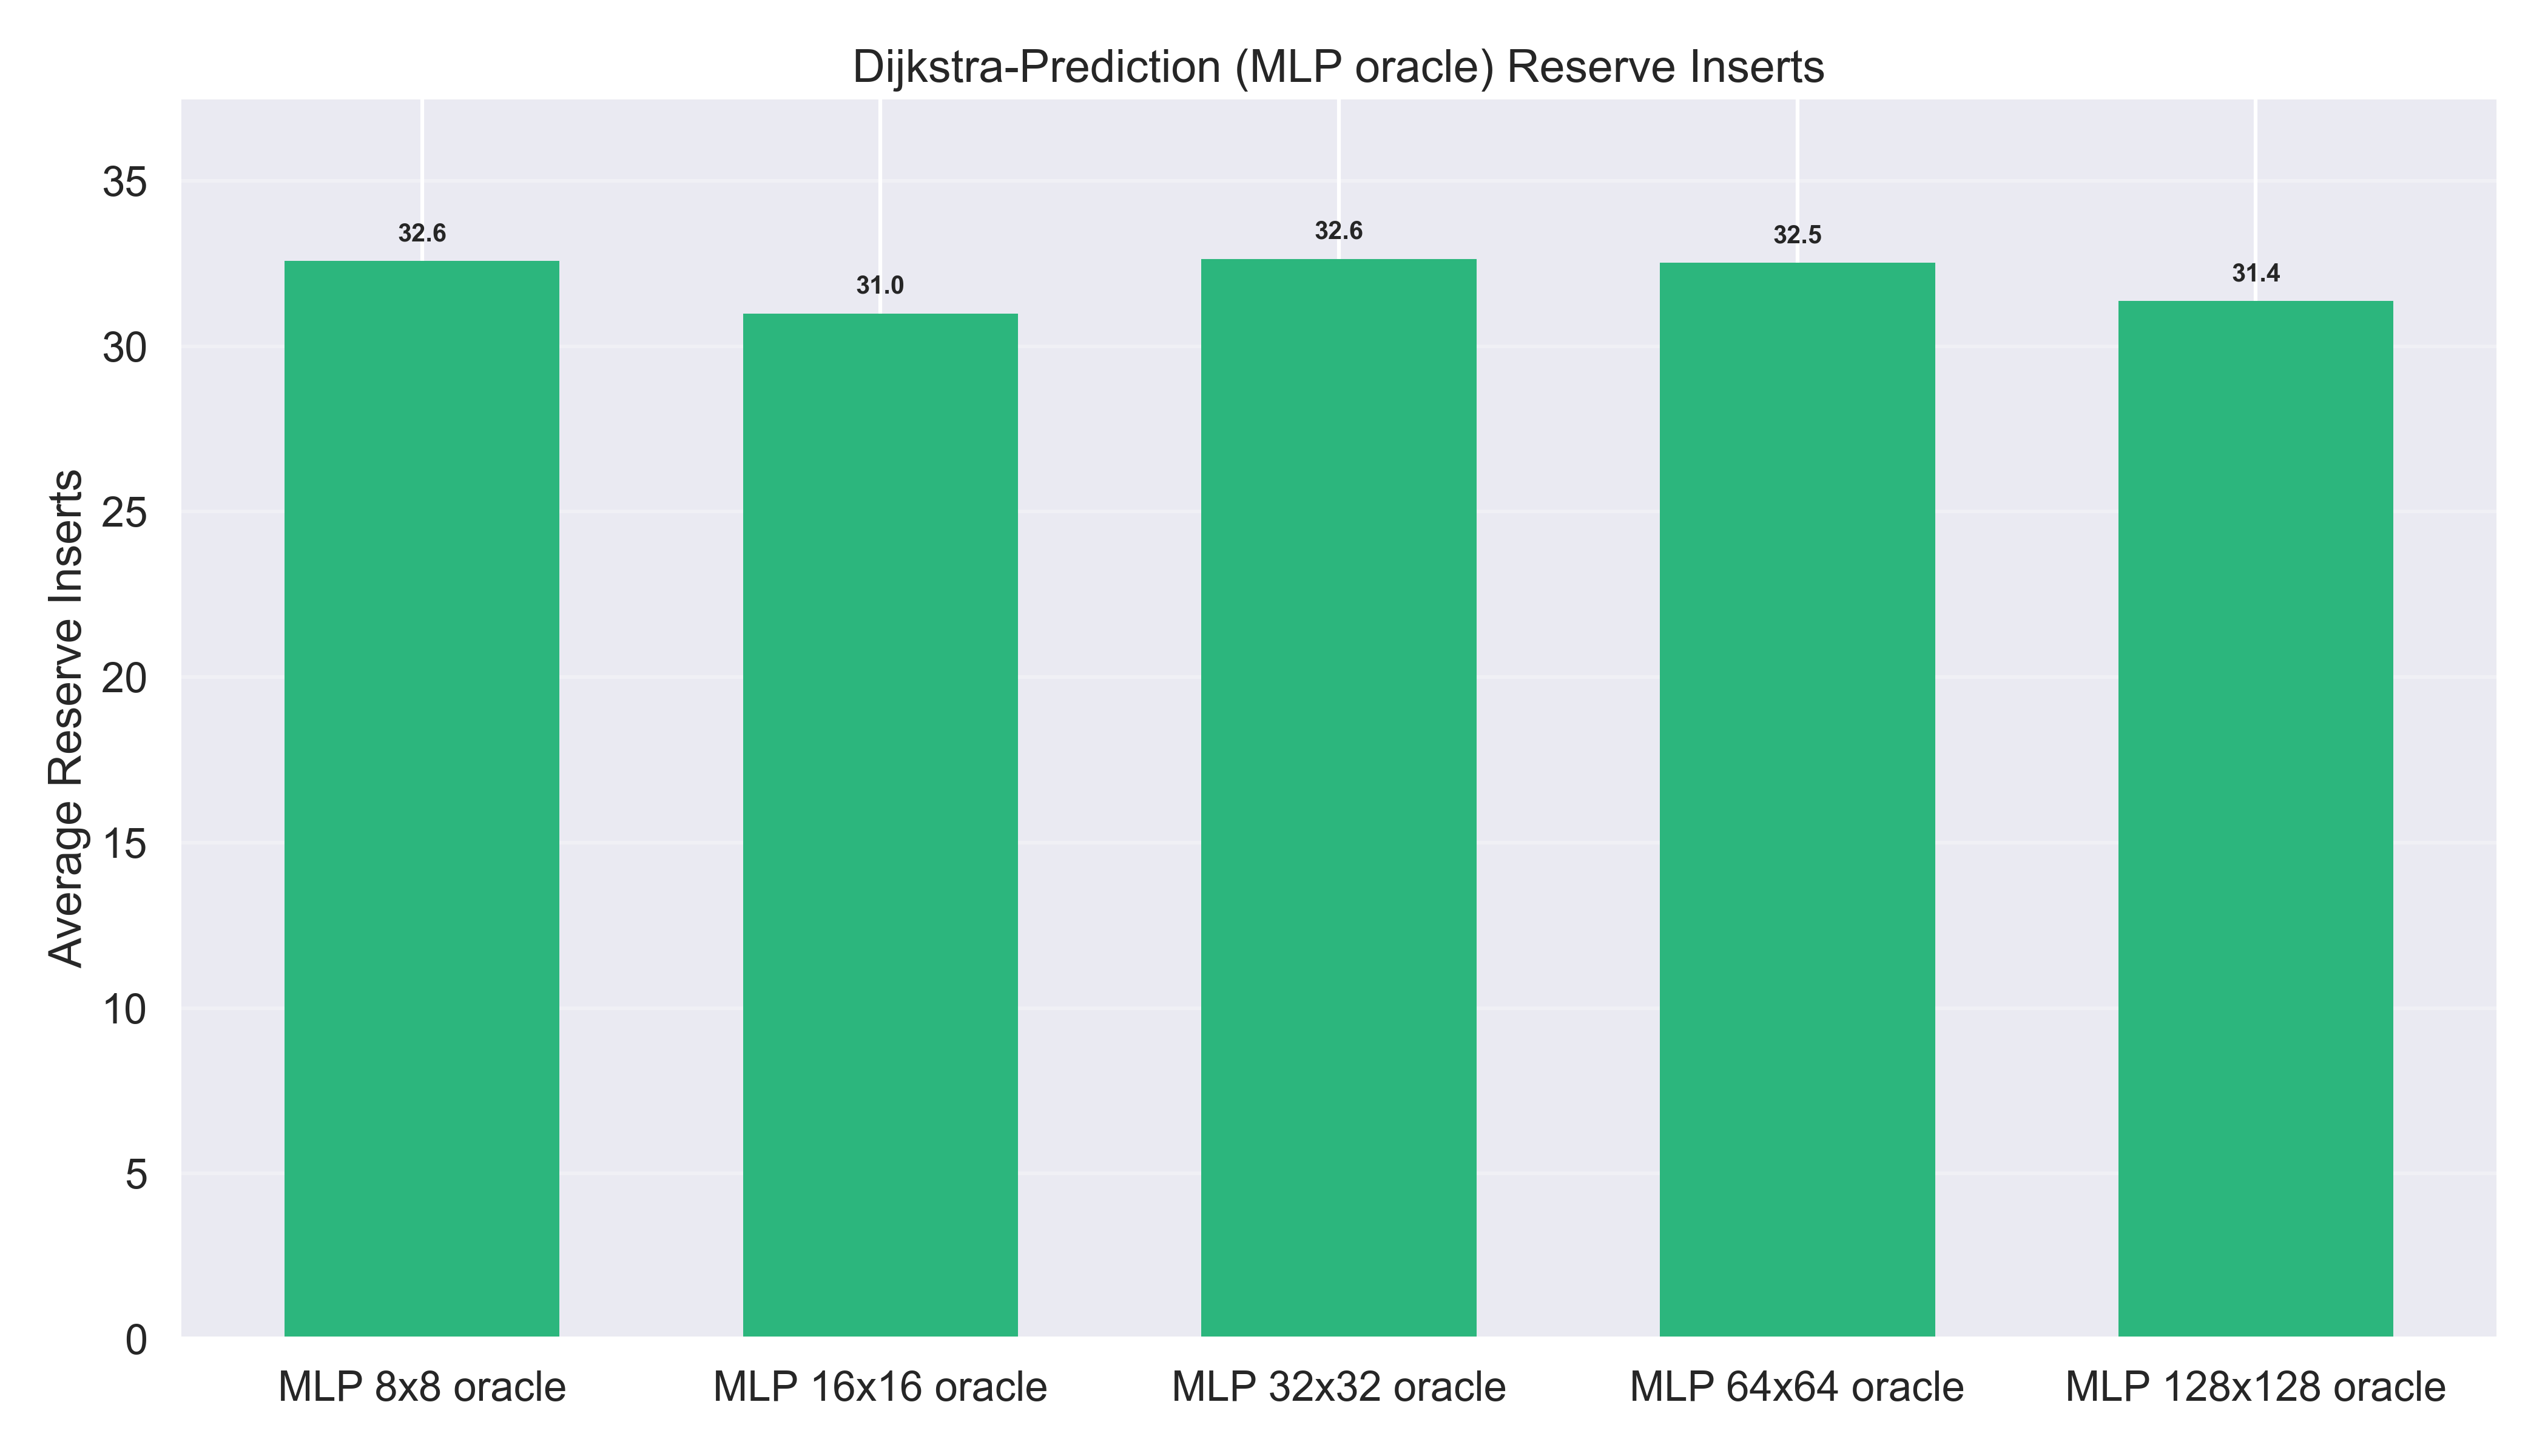
\includegraphics[width=1\linewidth]{tex/images/mlp_r_inserts_comparison.png}
    \caption{Average node insertions into the Reserve Set (MLP).}
    \label{fig:mlp_r_inserts}
\end{figure}

\begin{figure}[htbp]
    \centering
    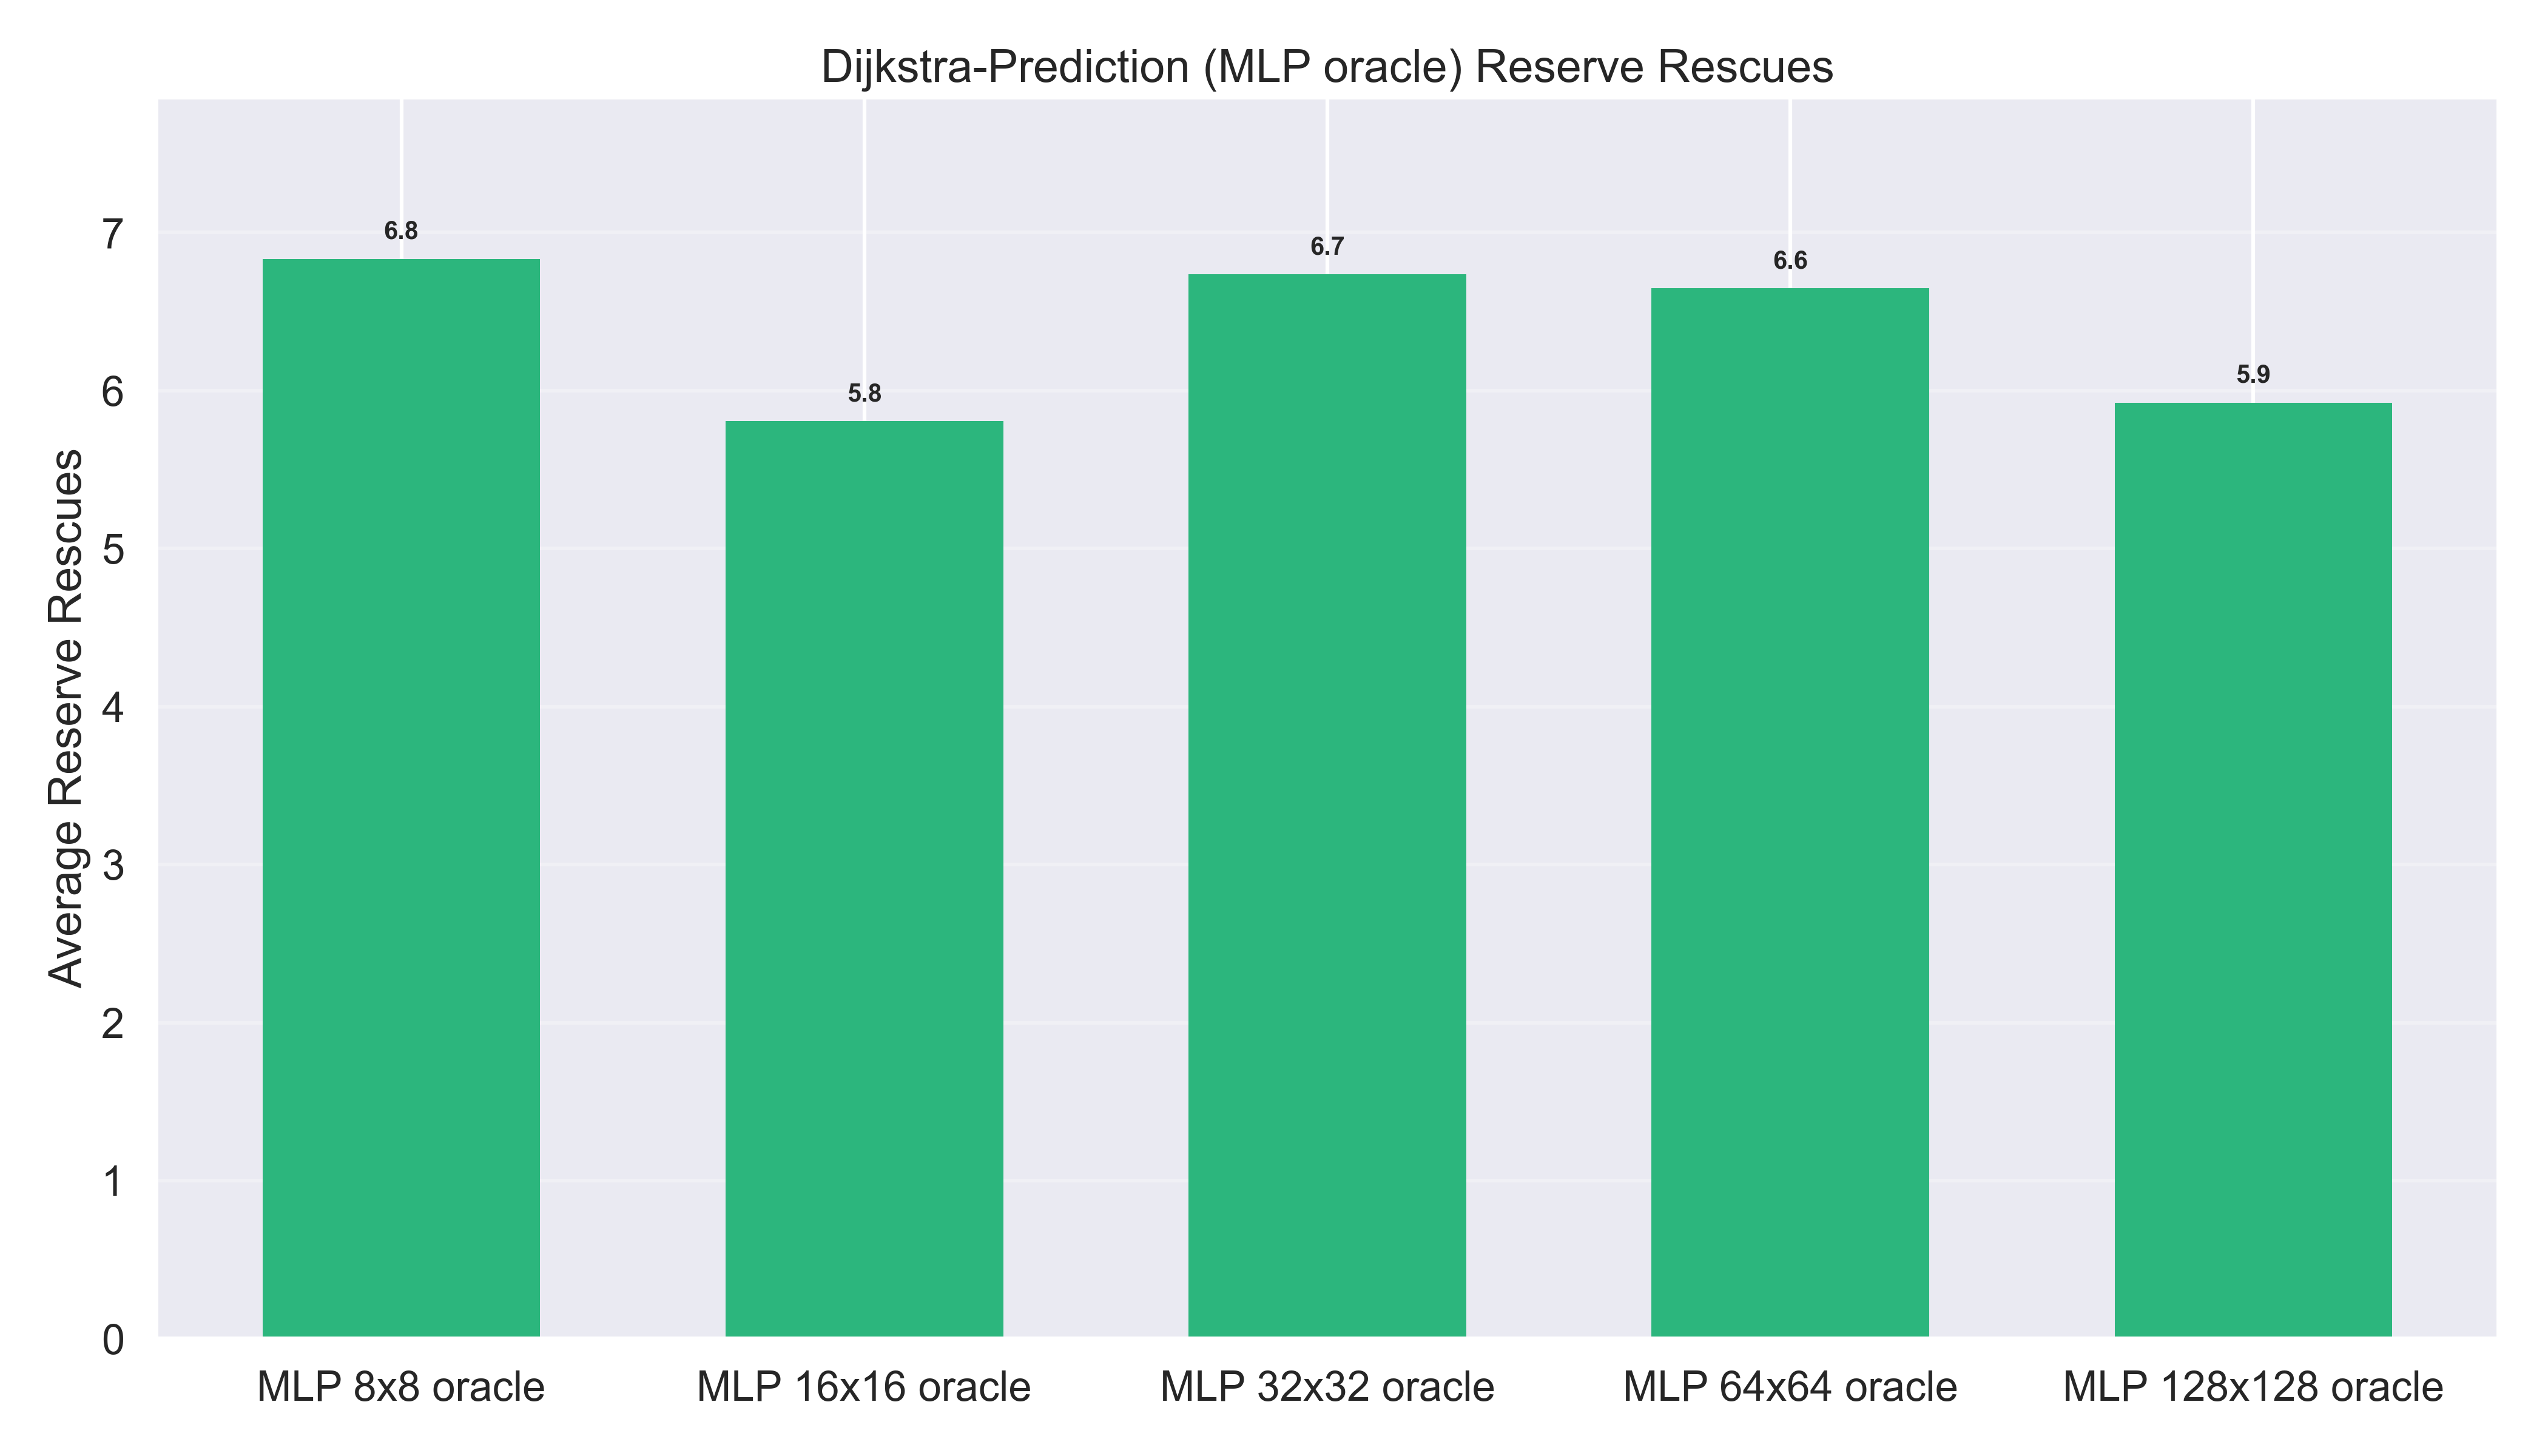
\includegraphics[width=1\linewidth]{tex/images/mlp_r_rescues_comparison.png}
    \caption{Average node rescues triggered during execution (MLP).}
    \label{fig:mlp_r_rescues}
\end{figure}

Similar to our previous observations, we conclude no significant distinction between the neural network size. Insertions into the Reserve Set ($R$) are $\approx32$, while rescues from the Set are $\approx6$.
\newpage

Finally, for the MLP oracles, we evaluated the average execution time per graph of the \texttt{DIJKSTRA-PREDICTION} algorithm in comparison to \texttt{DIJKSTRA}.
\vspace{1cm}

\begin{figure}[h]
    \centering
    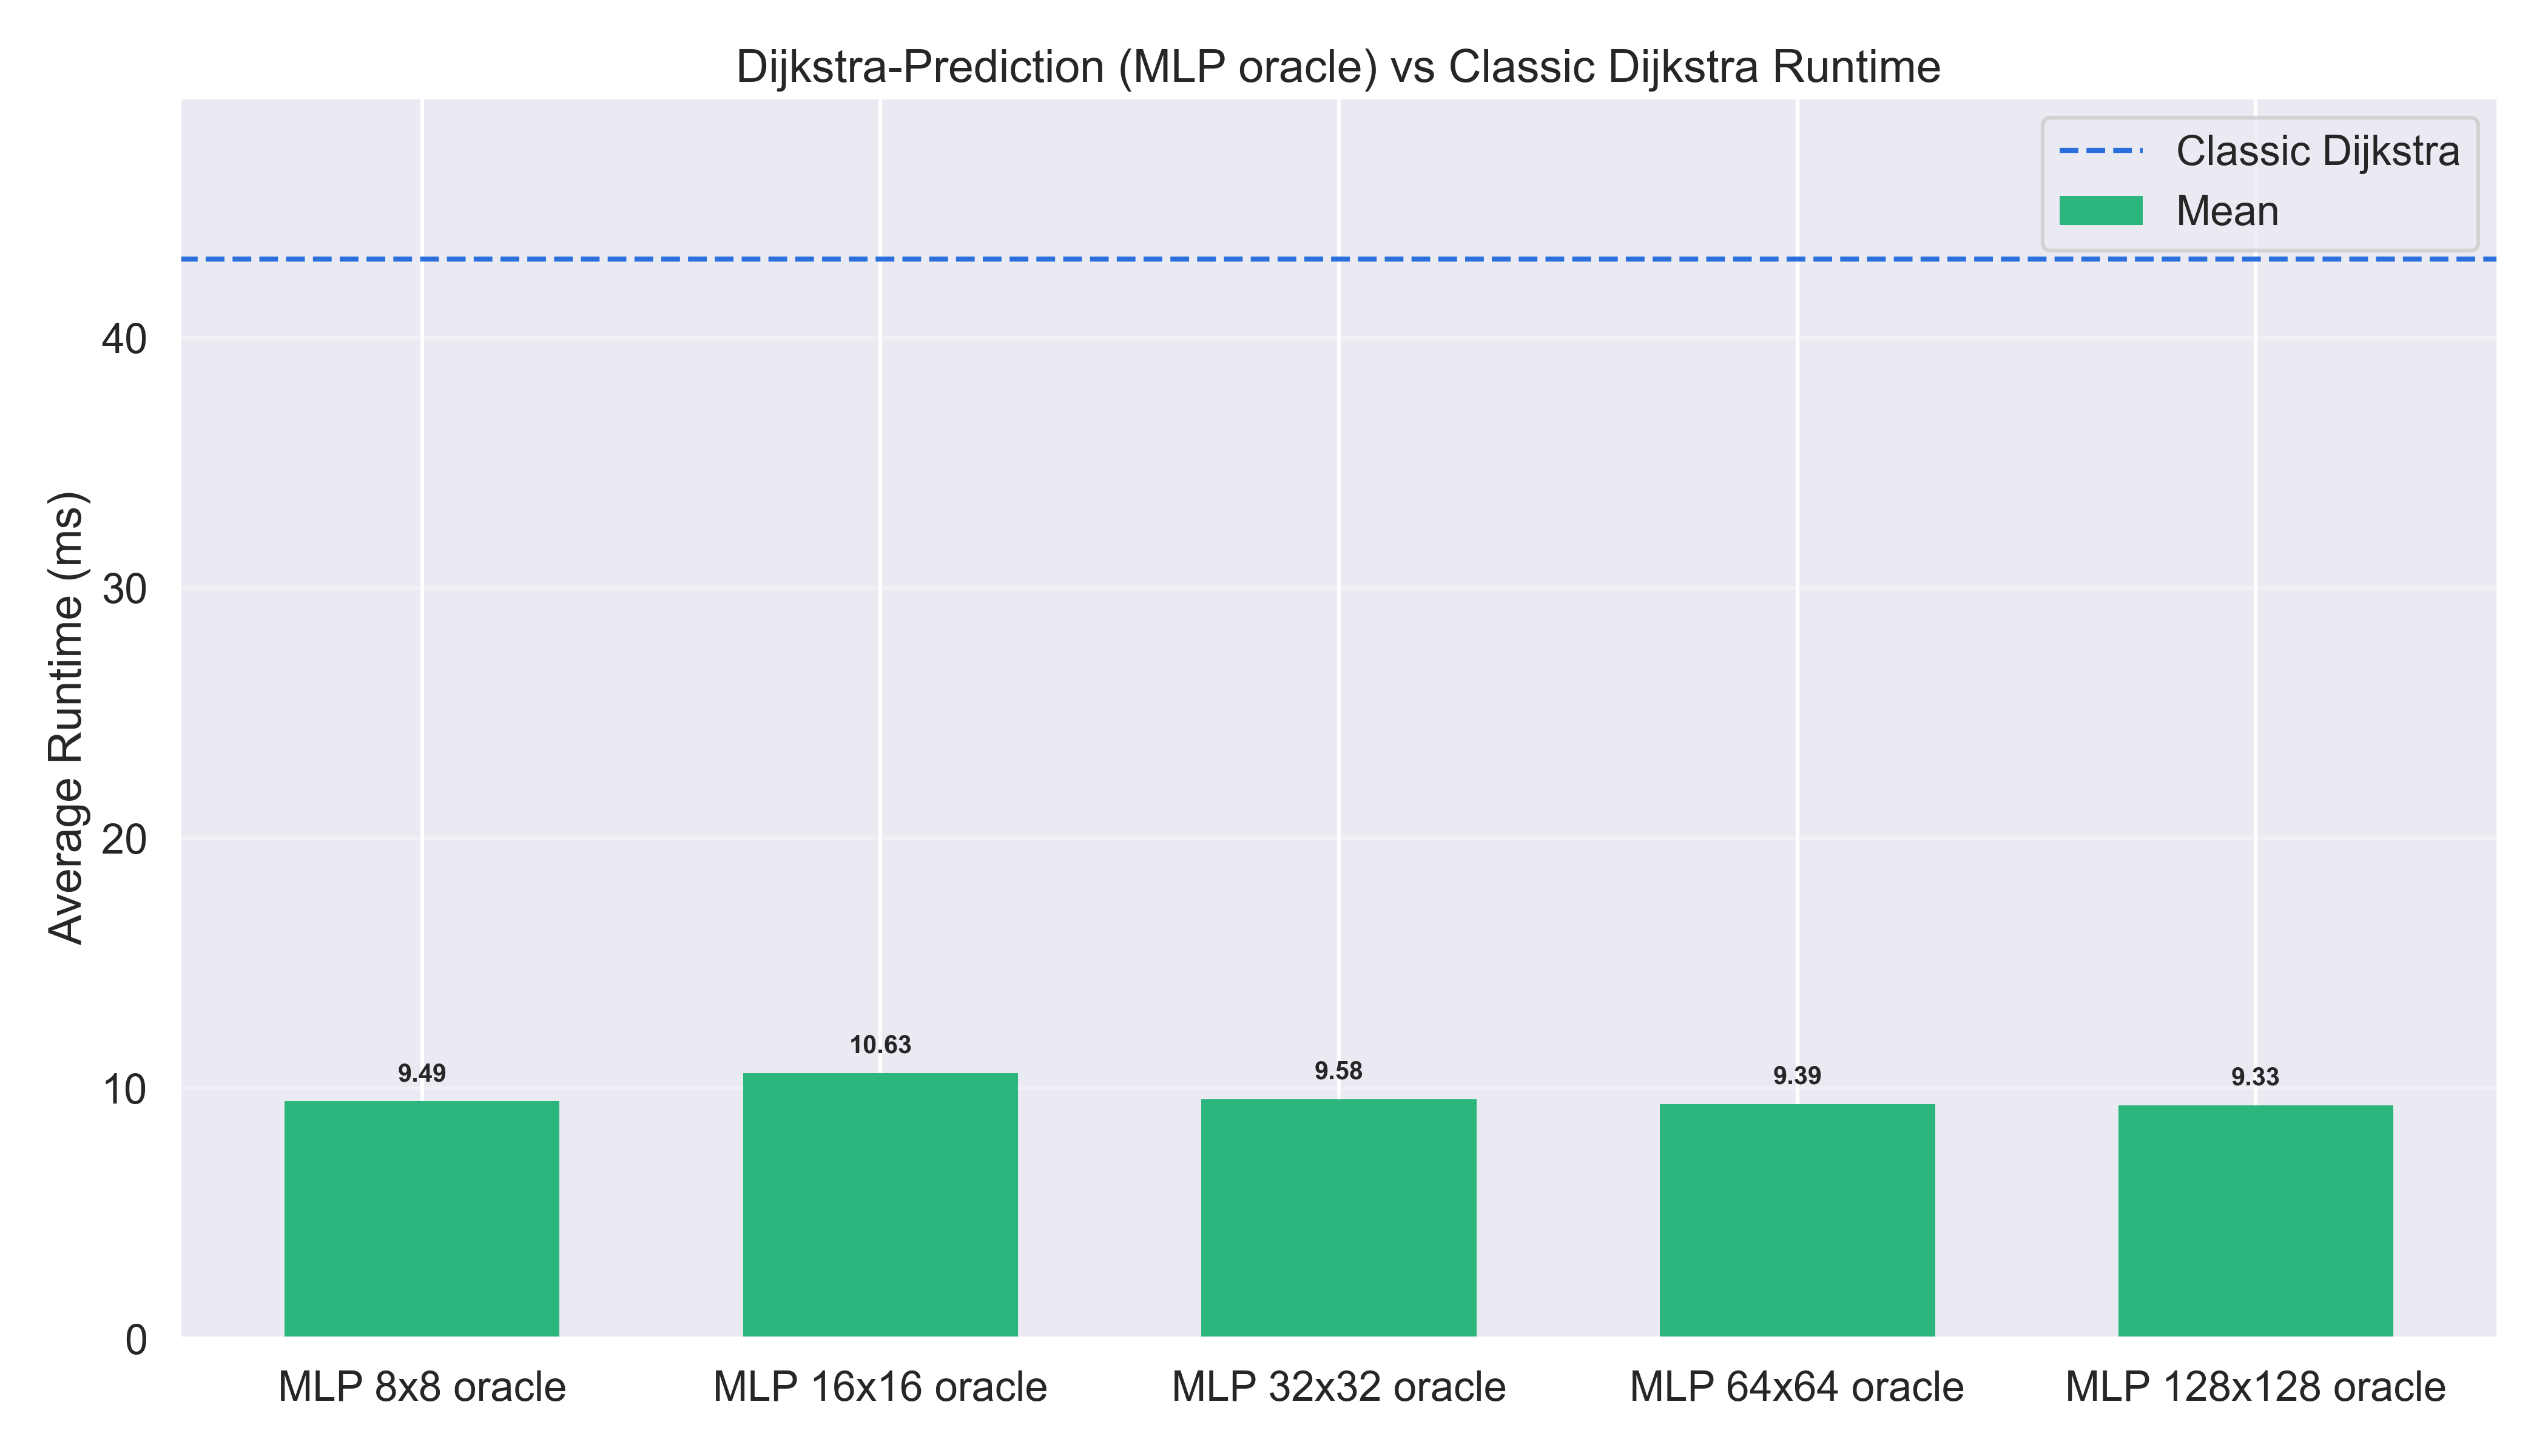
\includegraphics[width=1\linewidth]{tex/images/mlp_time_comparison.png}
    \caption{Average execution runtime (ms) for the MLP variants versus the classic approach}
    \label{fig:mlp_runtime}
\end{figure}
\newpage

\begin{table}[h]
\centering
\caption{Average Runtime (ms) with MLP oracle architectures.}
\label{tab:mlp_runtime}
\renewcommand{\tabularxcolumn}[1]{m{#1}}
\begin{tabularx}{\textwidth}{
    >{\centering\arraybackslash}X 
    >{\centering\arraybackslash}X 
}
\toprule
\textbf{Oracle Model Architecture} & \textbf{Average Runtime per Graph (ms)}  \\ \midrule
MLP(128x128) & 9.33 \\
MLP(64x64)   & 9.38 \\
MLP(32x32)   & 9.58 \\
MLP(16x16)   & 10.63 \\
MLP(8x8)     & 9.49 \\ \midrule
\texttt{DIJKSTRA} & 43.15  \\ \bottomrule
\end{tabularx}
\end{table}

The classic \texttt{DIJKSTRA} algorithm averaged a $43.15$ms execution time while the \texttt{DIJKSTRA-PREDICTION} algorithm achieved an average execution time of $\approx10$ms. The algorithm show a drop of more than \textbf{$75\%$}. Moreover, as shown in Table \ref{tab:mlp_runtime} and Figure \ref{fig:mlp_runtime}, we once again do not notice any significant distinction correlated to the scale of the neural network. We can attribute these minor fluctuations to system-level noise, hardware CPU scheduling, the Python interpreter, and background optimization tasks leading to small variations.

\subsection{Algorithmic Execution of XGBoost Oracle Architectures}
\label{subsec:xgboost_benchmark}

Following the evaluation of the neural networks, we bench-marked the tree-based ensemble models. As previously stated (See \ref{subsec:xgboost_training}), while XGBoost models are unviable for extrapolation, in theory they are still well suited for specific environments.

Table \ref{tab:xgboost_prio} and Figures \ref{fig:xgboost_prio} and \ref{fig:xgboost_skipped_prio} detail the average priority queue operations compared to the classic \texttt{DIJKSTRA} algorithm, highlighting the operations successfully skipped by the gradient boosting variants.

\begin{figure}[htbp]
    \centering
    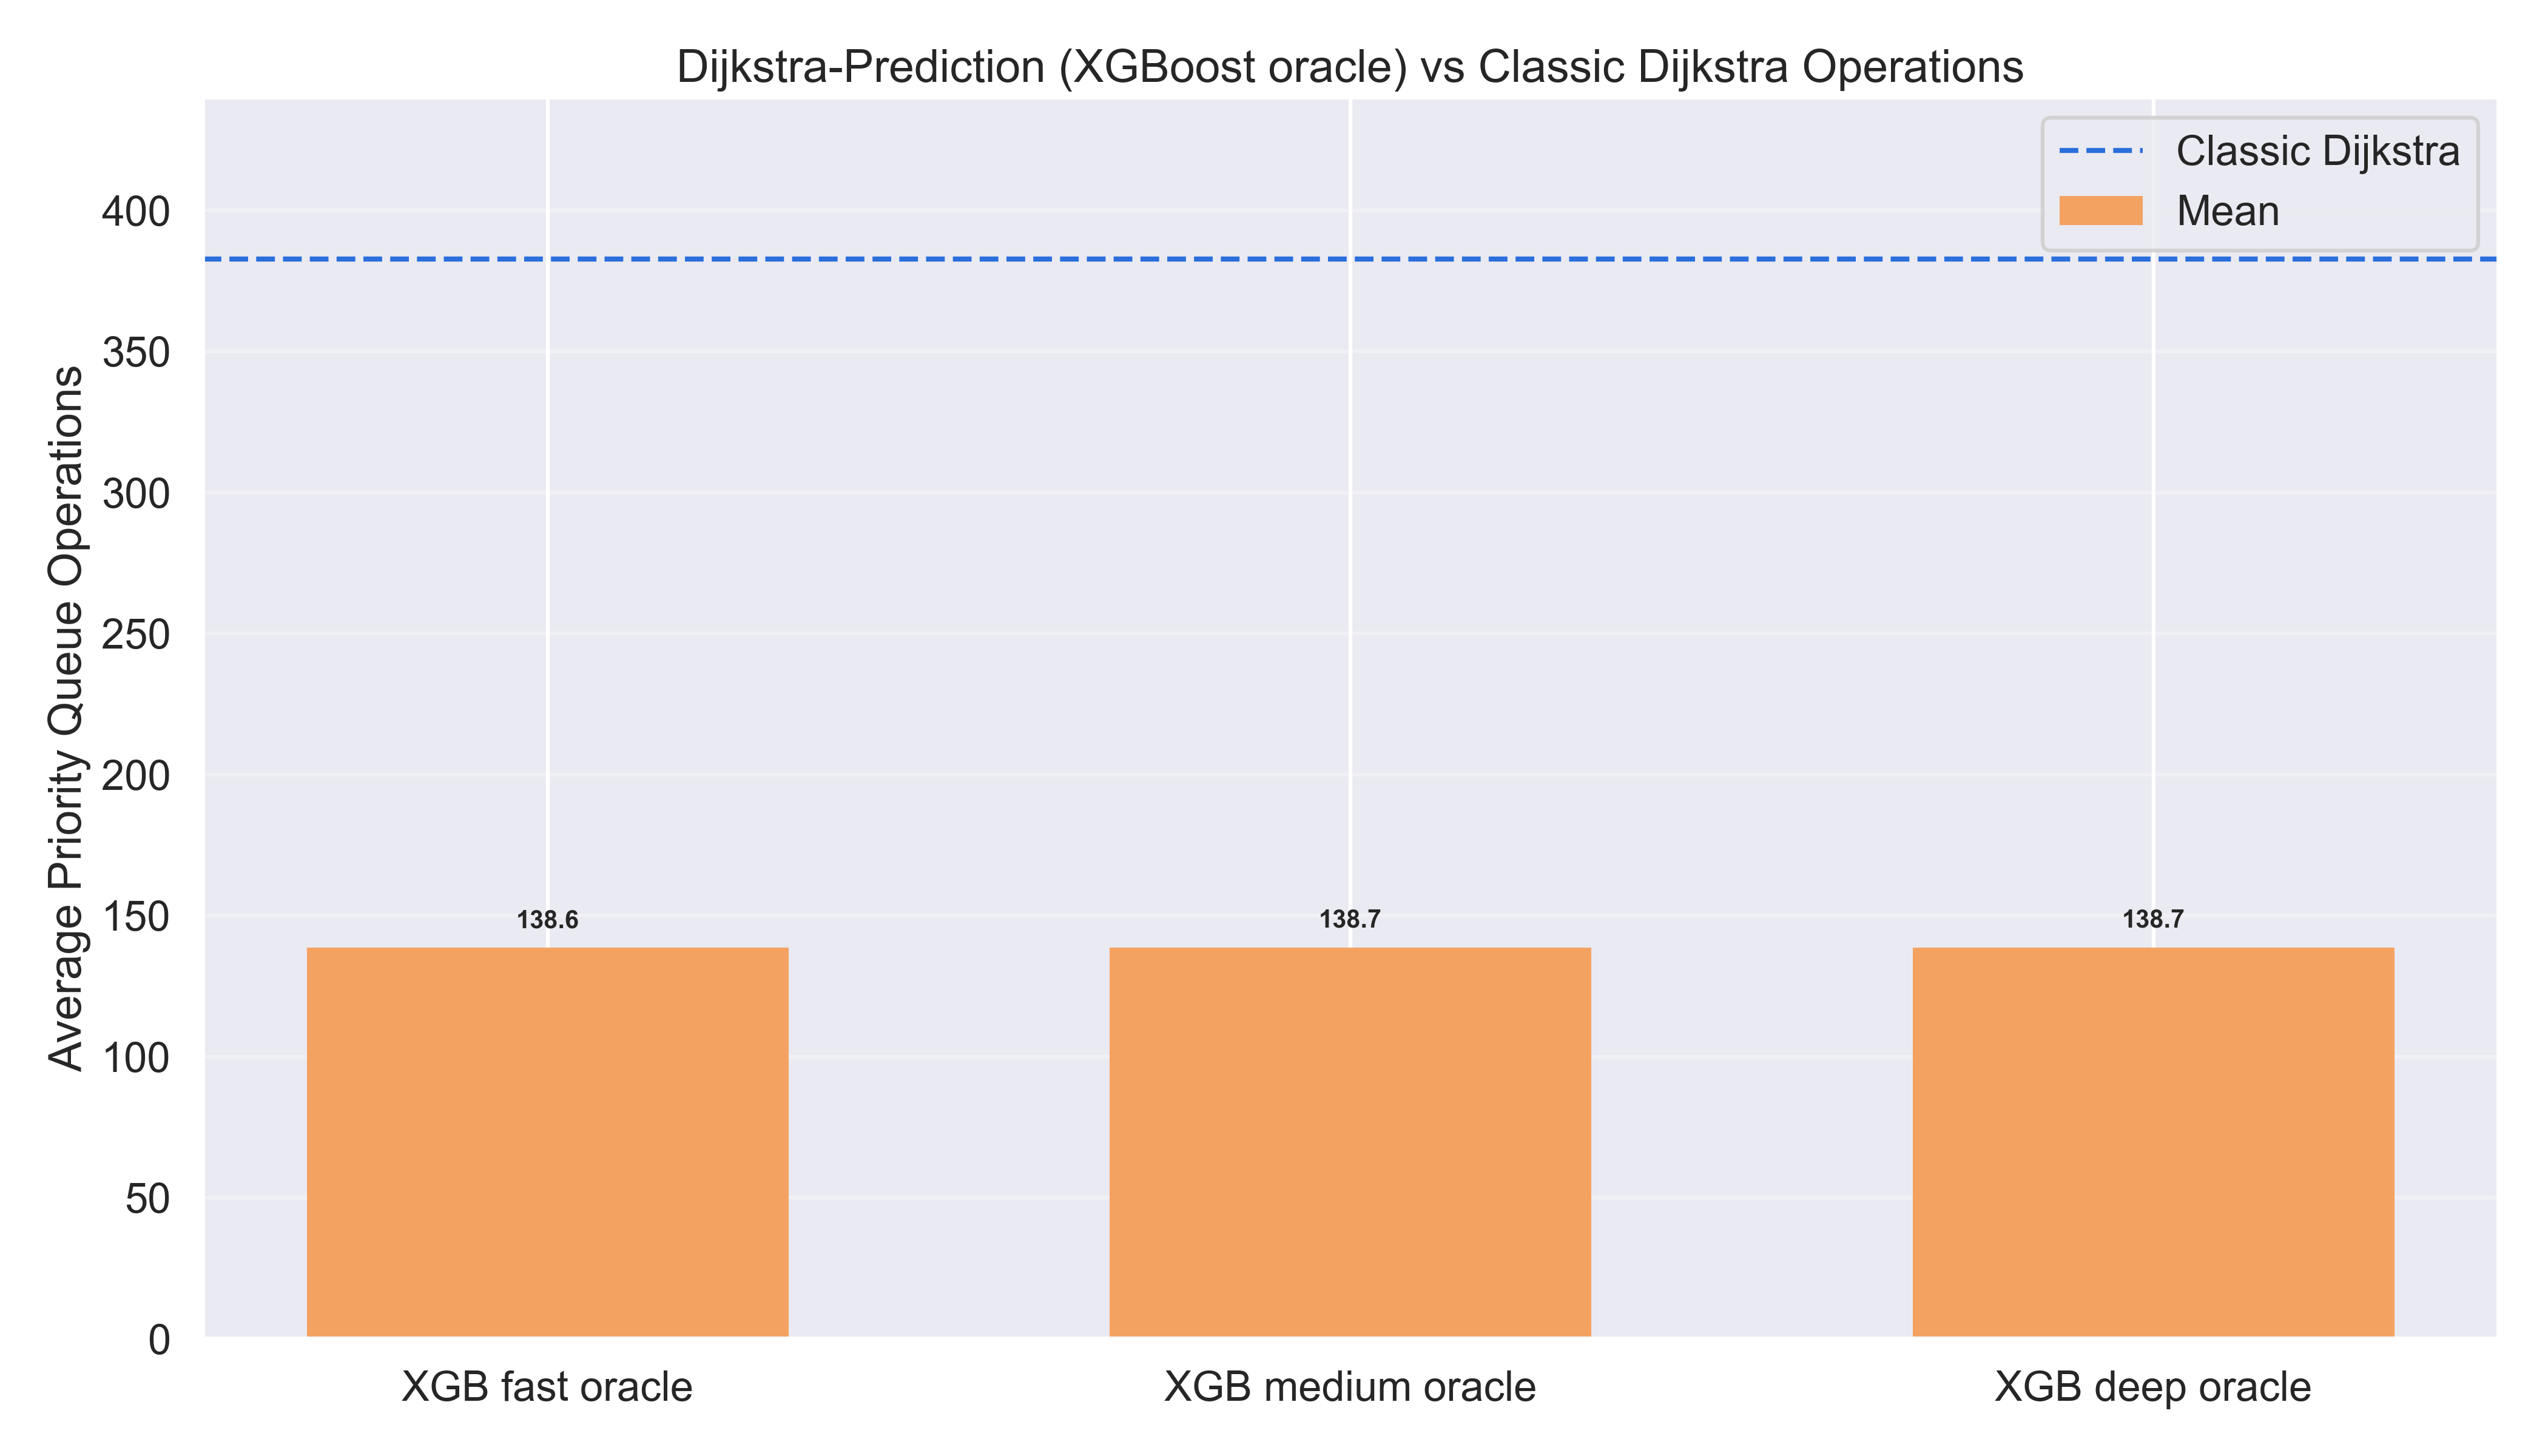
\includegraphics[width=1\linewidth]{tex/images/xgb_ops_comparison.png}
    \caption{Average operations achieved via prediction pruning (XGBoost).}
    \label{fig:xgboost_prio}
\end{figure}

\begin{figure}[htbp]
    \centering
    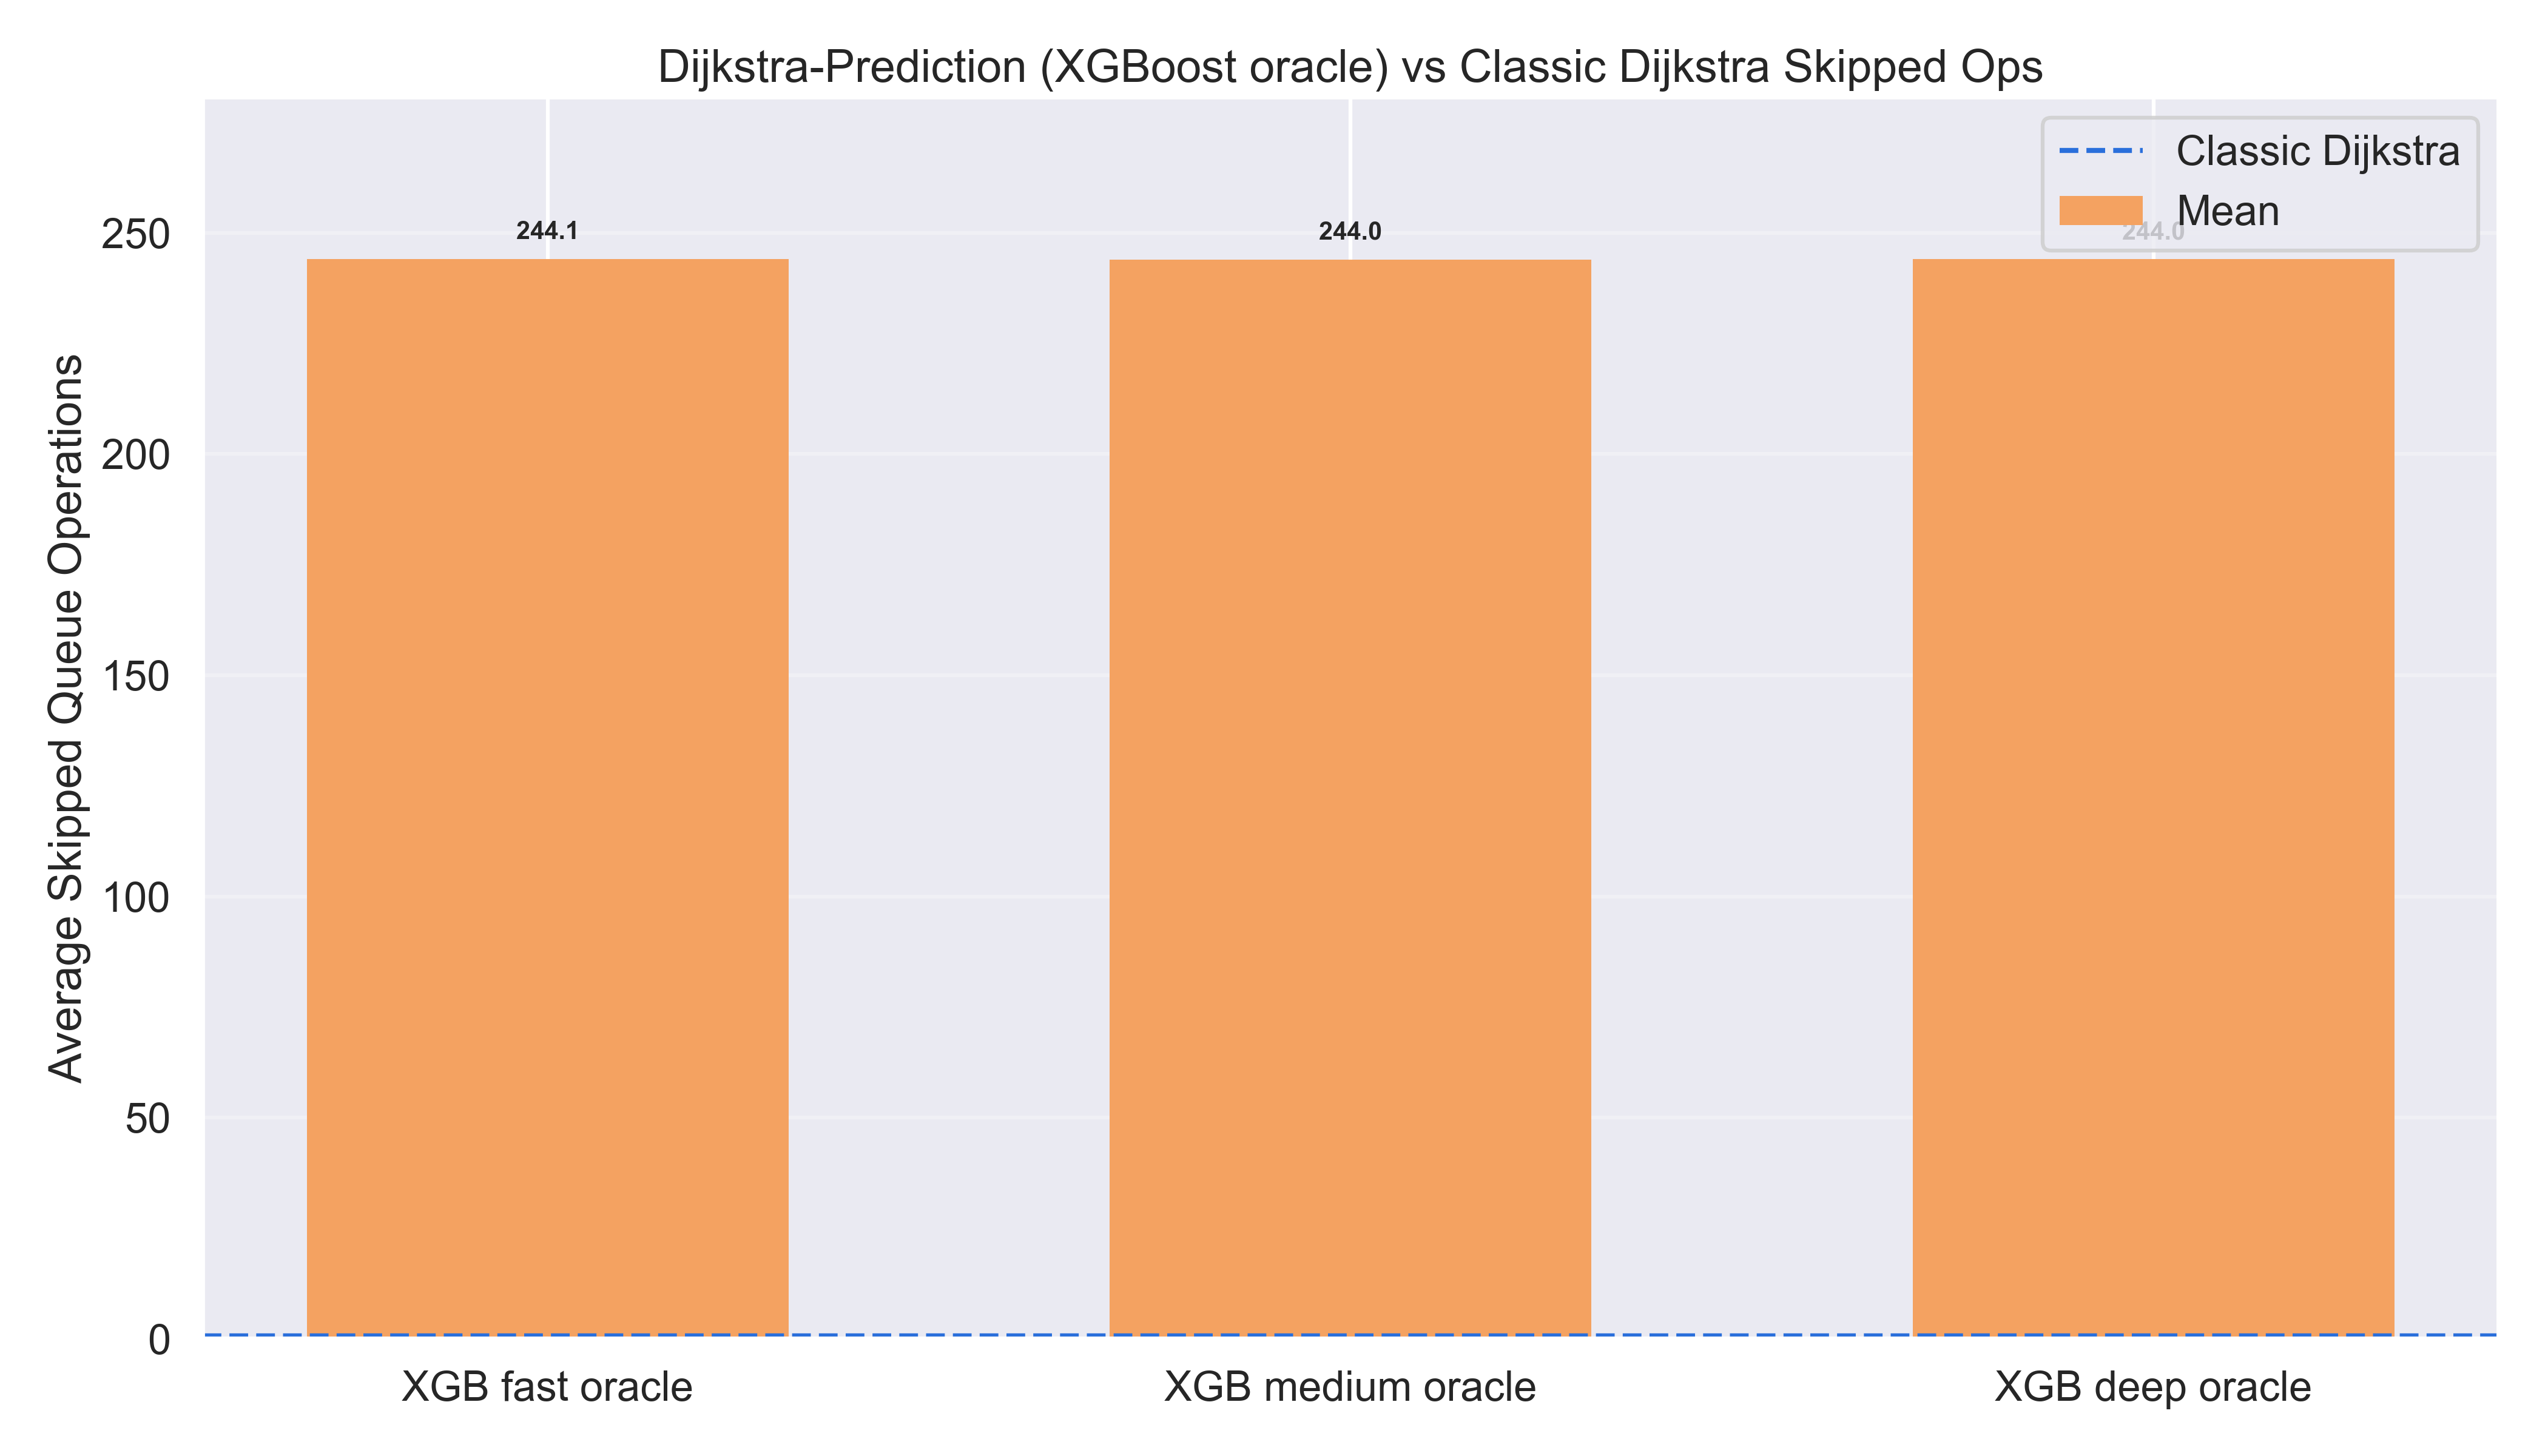
\includegraphics[width=1\linewidth]{tex/images/xgb_skipped_ops_comparison.png}
    \caption{Average skipped operations achieved via prediction pruning (XGBoost).}
    \label{fig:xgboost_skipped_prio}
\end{figure}
\newpage

\begin{table}[h]
\centering
\caption{Priority Queue Operations with XGBoost oracle architectures.}
\label{tab:xgboost_prio}
\renewcommand{\tabularxcolumn}[1]{m{#1}}
\begin{tabularx}{\textwidth}{
    >{\centering\arraybackslash}X 
    >{\centering\arraybackslash}X 
    >{\centering\arraybackslash}X
}
\toprule
\textbf{Oracle Model Architecture} & \textbf{Average Priority Queue Operations} & \textbf{Average Priority Queue Operation Skips} \\ \midrule
XGBoost Deep (300,5,0.05)  & 138.68 & 244.01 \\
XGBoost Medium (200,4,0.05) & 138.71 & 243.98 \\
XGBoost Fast (100,3,0.1)  & 138.64 & 244.05 \\ \midrule
\texttt{DIJKSTRA} & 382.7 & - \\ \bottomrule
\end{tabularx}
\end{table}

Similar to the MLP oracle architecture, \texttt{DIJKSTRA-PREDICTION} sees a large reduction in priority queue operations with the XGBoost oracle architecture. More specifically, All variants average $\approx138.7$ operations per graph compared to to an average of 382.7 operations per graph achieved by the classic \texttt{DIJKSTRA} algorithm.

Table \ref{tab:xgboost_reserve} alongside Figures \ref{fig:xgboost_r_inserts} and \ref{fig:xgboost_r_rescues}, showcase the frequency of the Reserve Set ($R$) operations.

\begin{figure}[htbp]
    \centering
    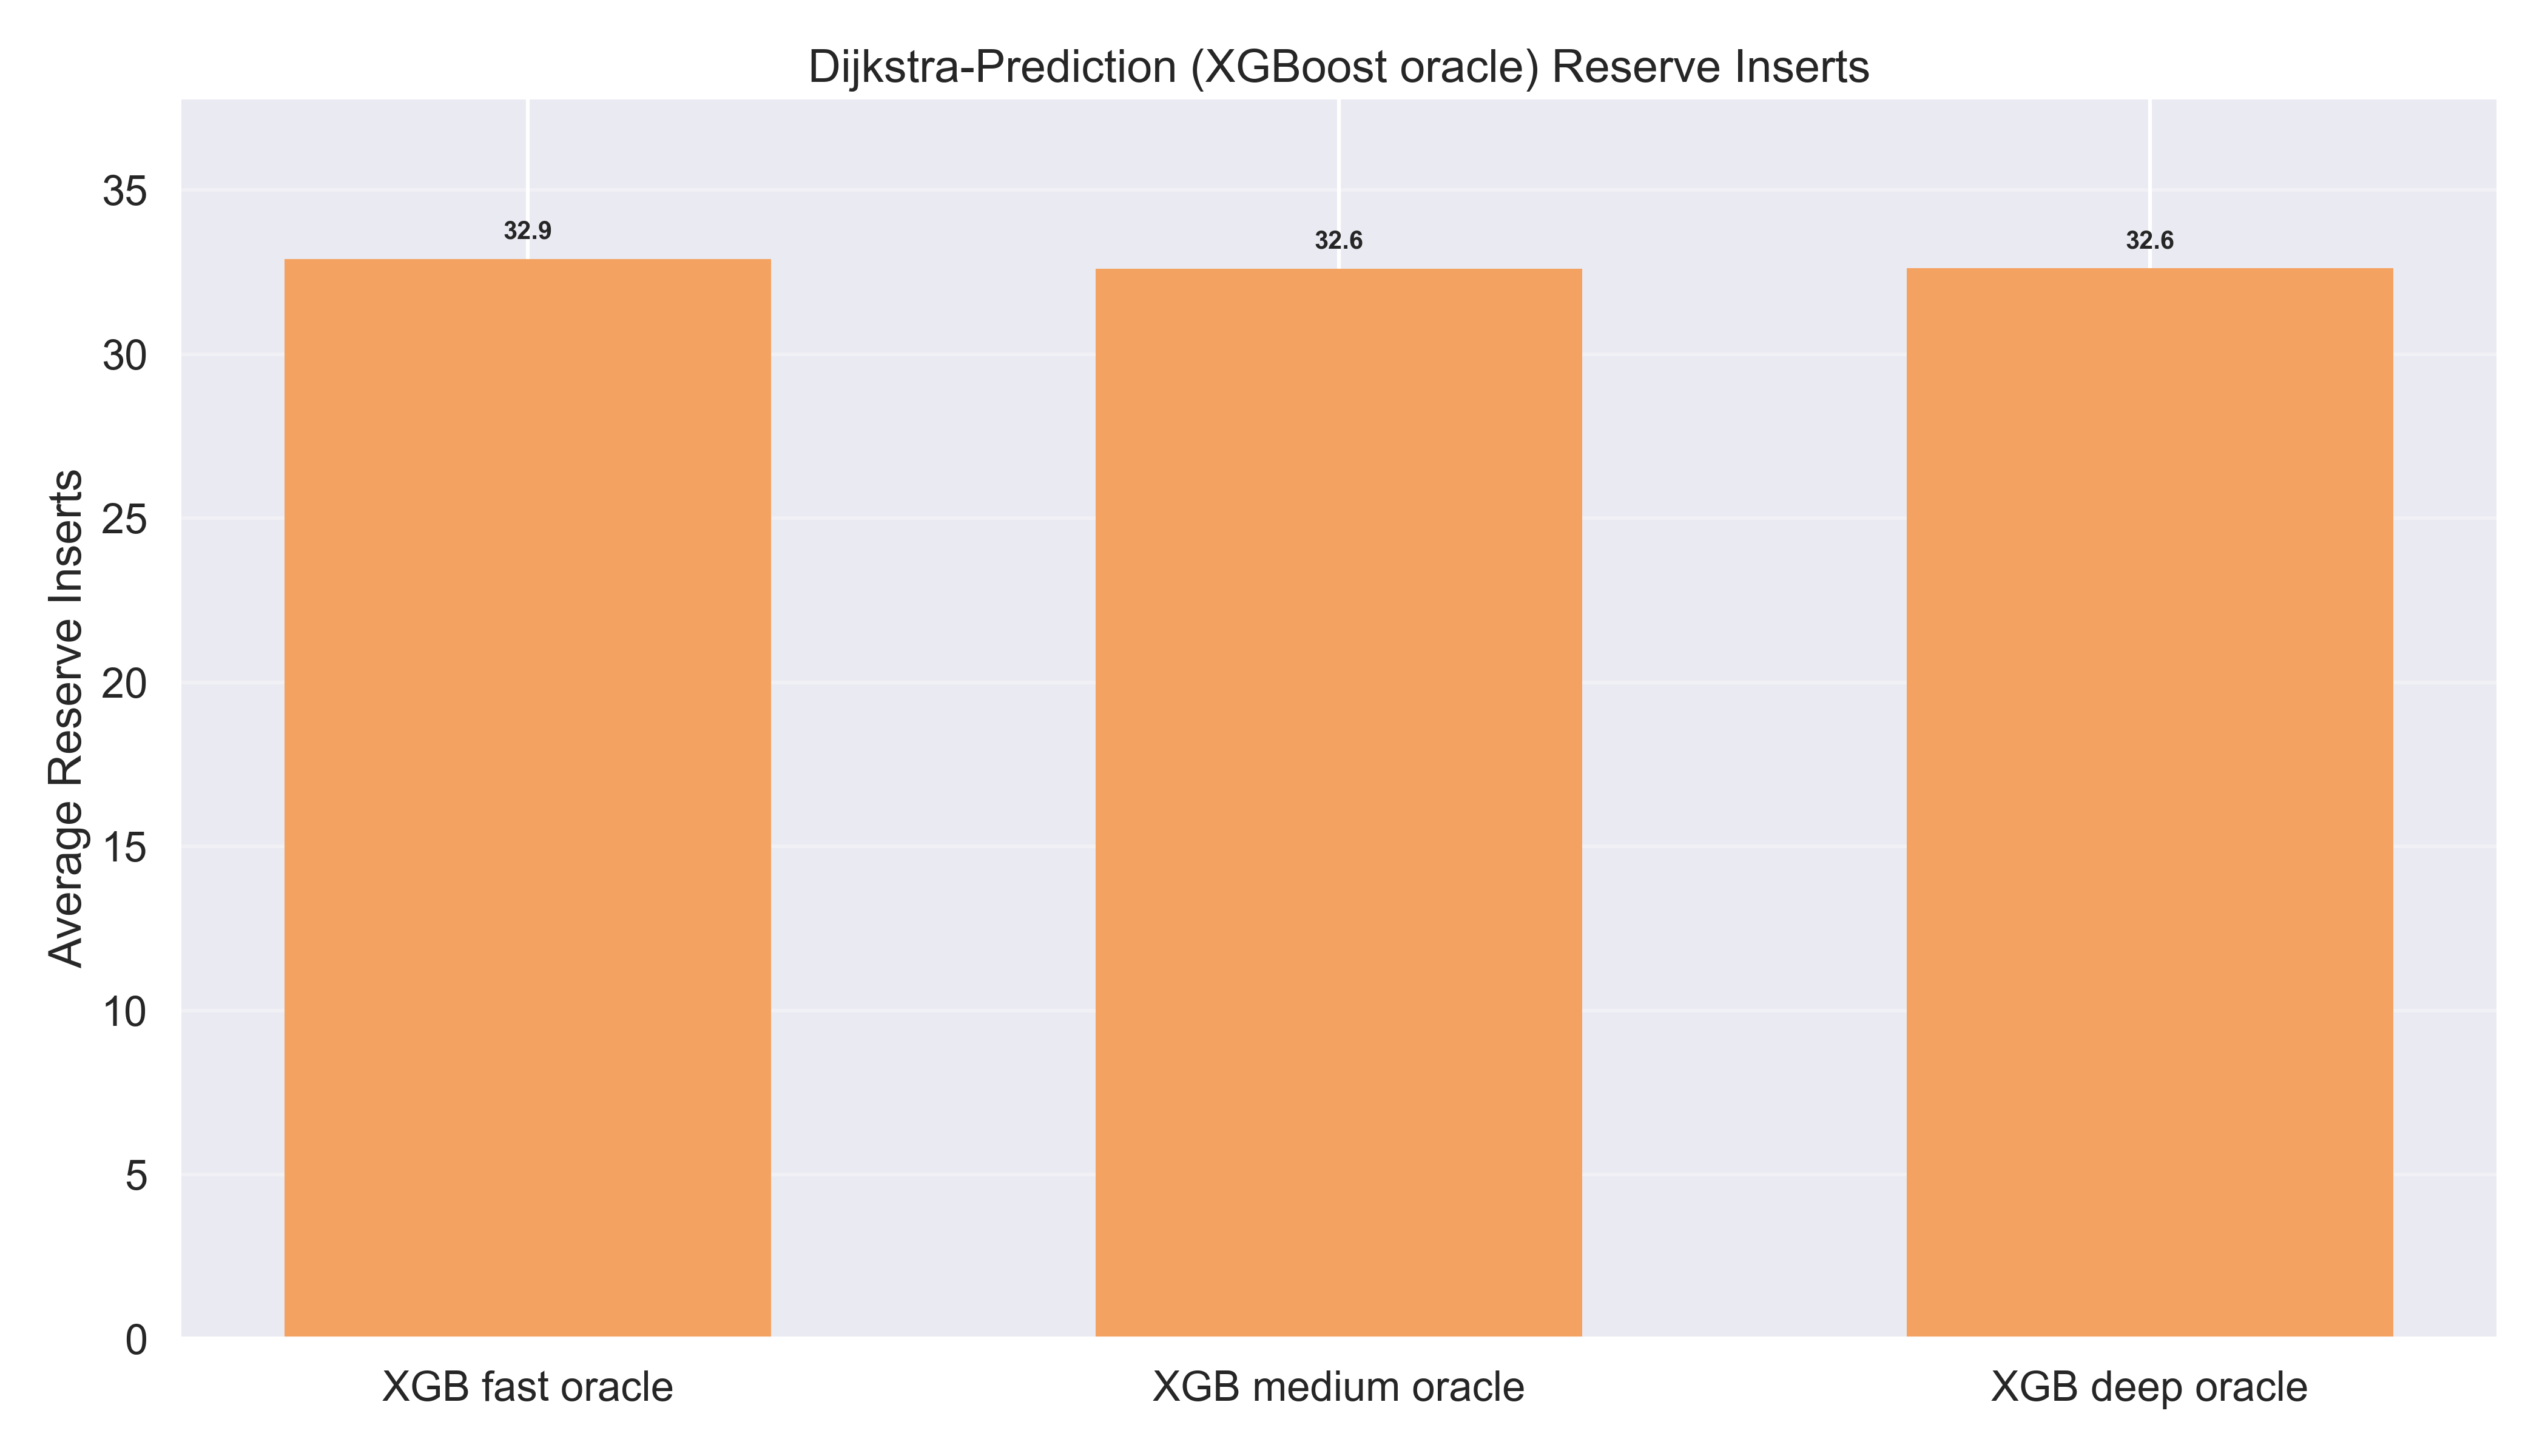
\includegraphics[width=1\linewidth]{tex/images/xgb_r_inserts_comparison.png}
    \caption{Average node insertions into the Reserve Set (XGBoost).}
    \label{fig:xgboost_r_inserts}
\end{figure}

\begin{figure}[htbp]
    \centering
    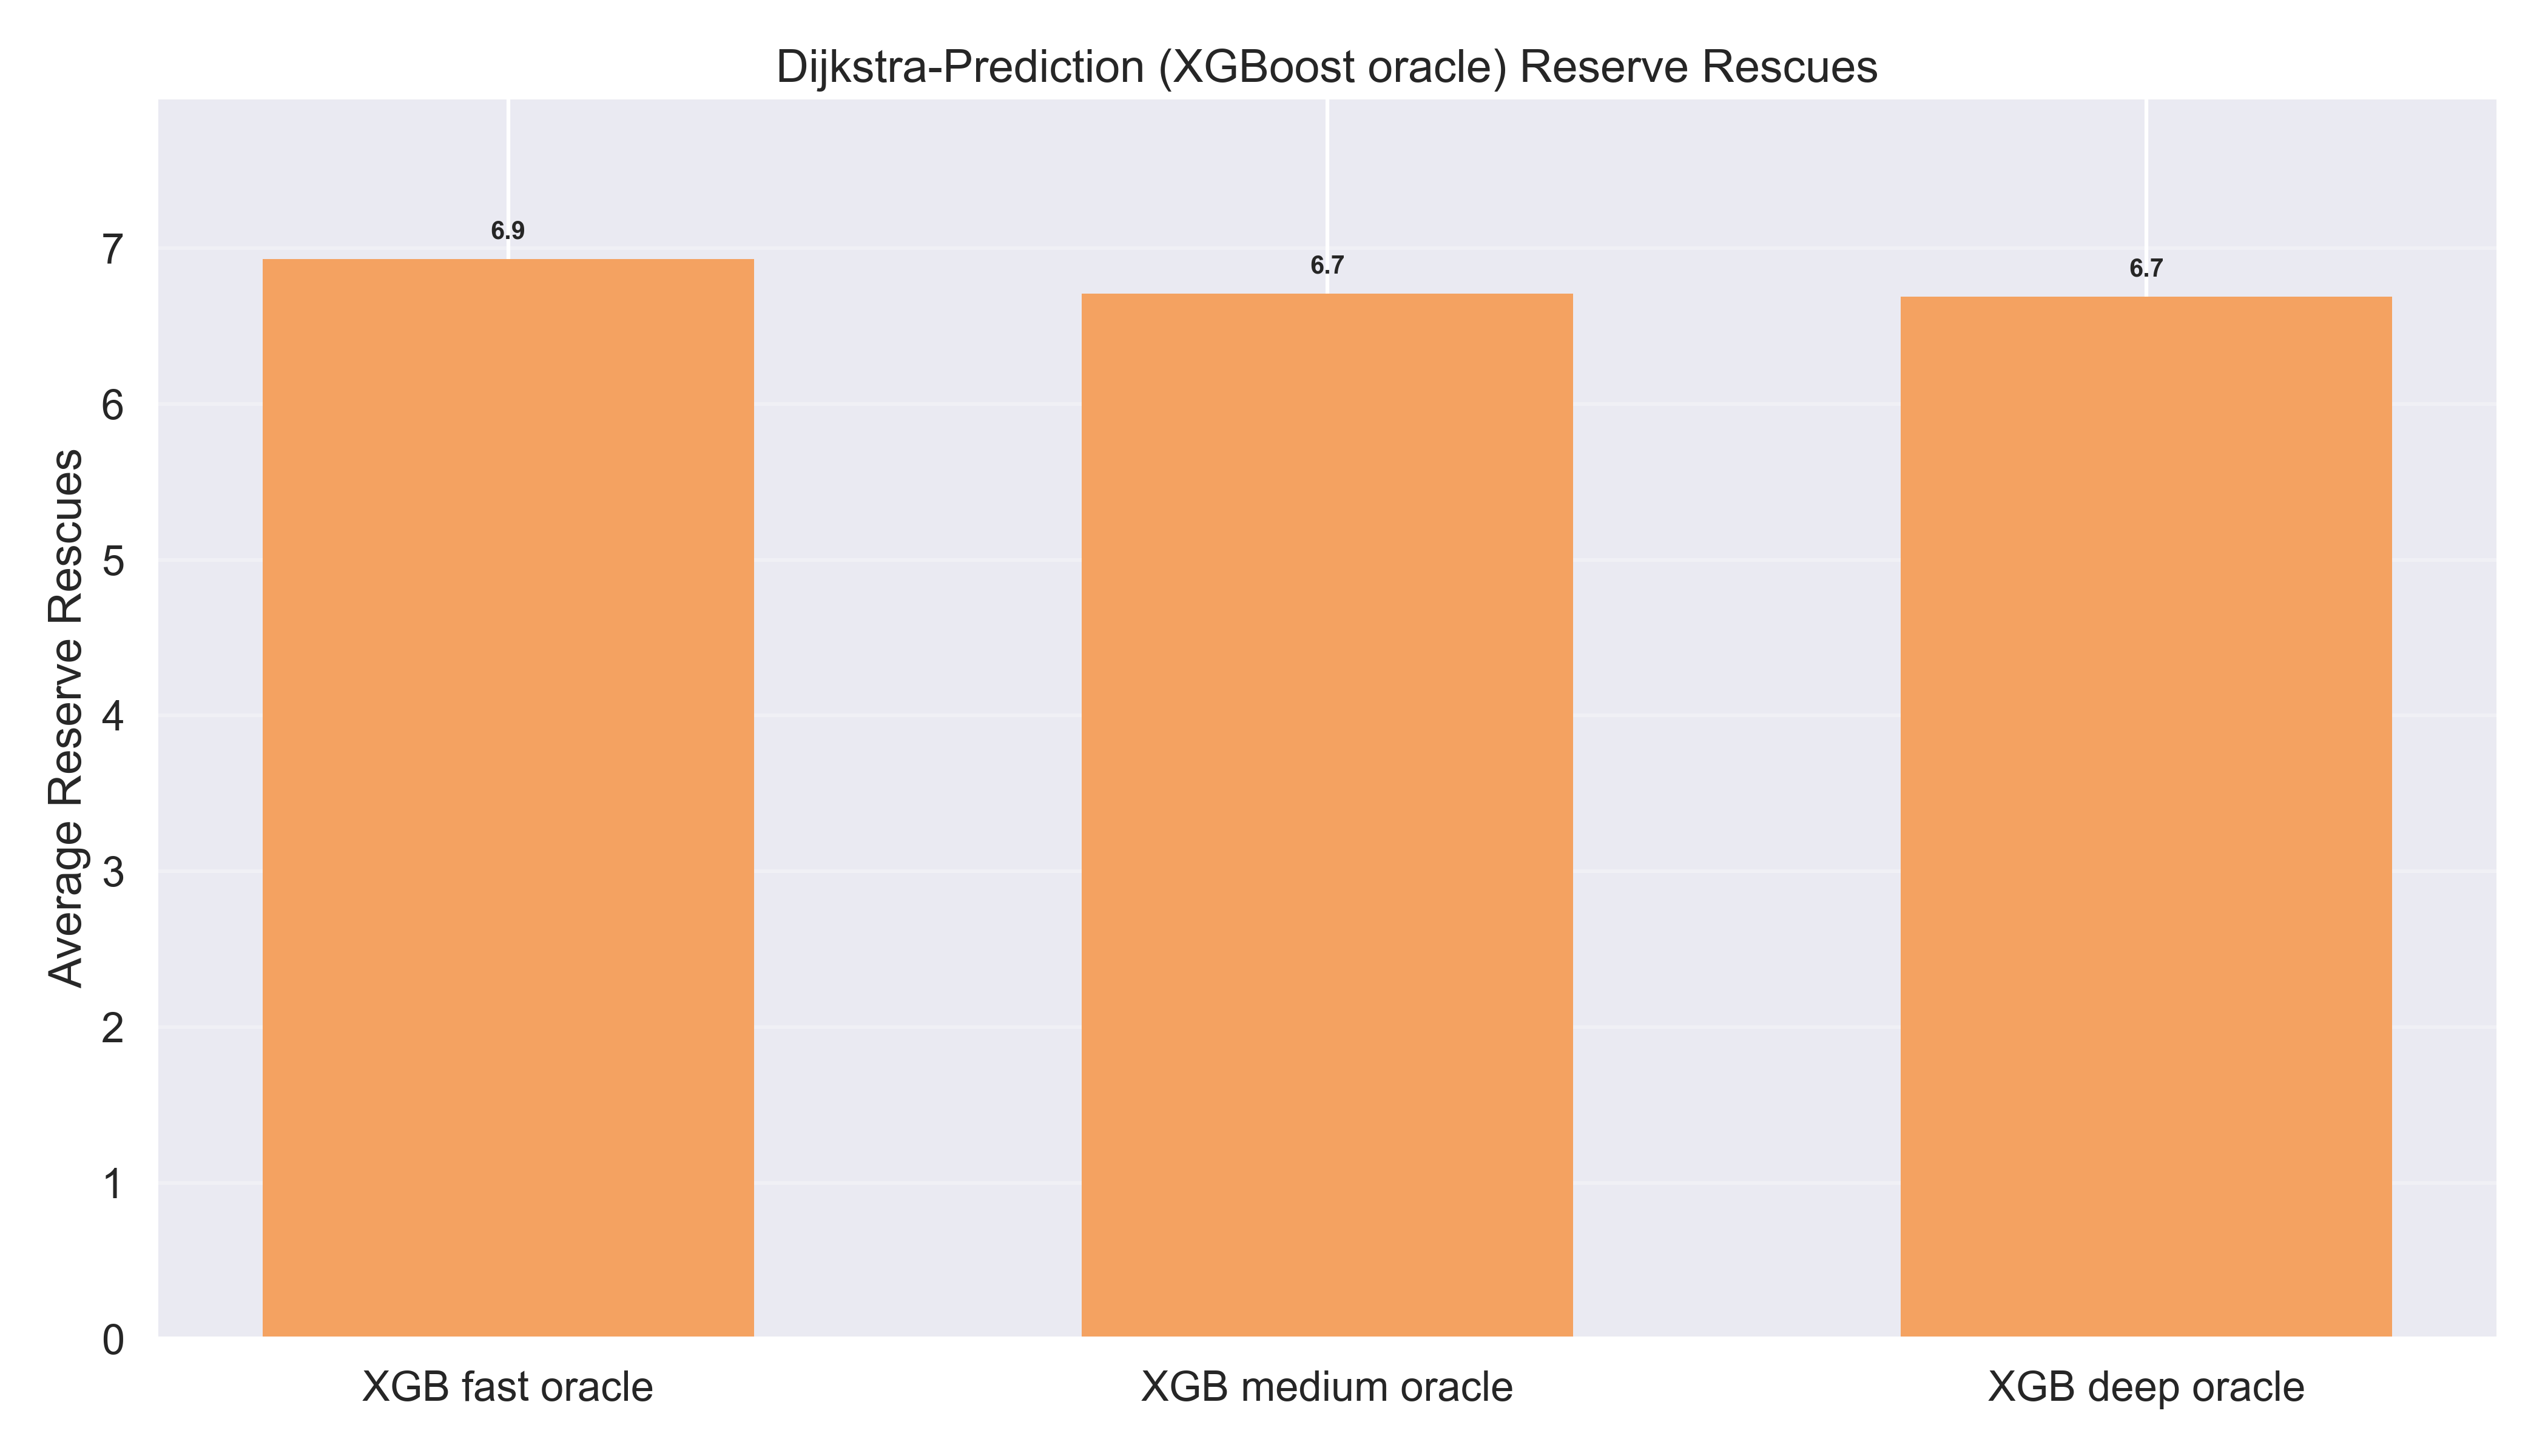
\includegraphics[width=1\linewidth]{tex/images/xgb_r_rescues_comparison.png}
    \caption{Average node rescues triggered during execution (XGBoost).}
    \label{fig:xgboost_r_rescues}
\end{figure}

\begin{table}[h]
\centering
\caption{Reserve Set Operations with XGBoost oracle architectures.}
\label{tab:xgboost_reserve}
\renewcommand{\tabularxcolumn}[1]{m{#1}}
\begin{tabularx}{\textwidth}{
    >{\centering\arraybackslash}X 
    >{\centering\arraybackslash}X 
    >{\centering\arraybackslash}X
}
\toprule
\textbf{Oracle Model Architecture} & \textbf{Average Reserve Set Inserts} & \textbf{Average Reserve Set Rescues} \\ \midrule
XGBoost Deep (300,5,0.05)  & 32.61 & 6.68 \\
XGBoost Medium (200,4,0.05) & 32.90 & 6.70 \\
XGBoost Fast (100,3,0.1)  & 32.61 & 6.92 \\ \bottomrule
\end{tabularx}
\end{table}
\newpage

The XGBoost models result in near-identical results to the MLP metrics with $\approx32.7$ node insertions and $\approx6.7$ rescues per graph.

Finally, we analyze the average execution time of the algorithm utilizing XGBoost models in Table \ref{tab:xgboost_runtime} and Figure \ref{fig:xgboost_runtime}.

\begin{figure}[h]
    \centering
    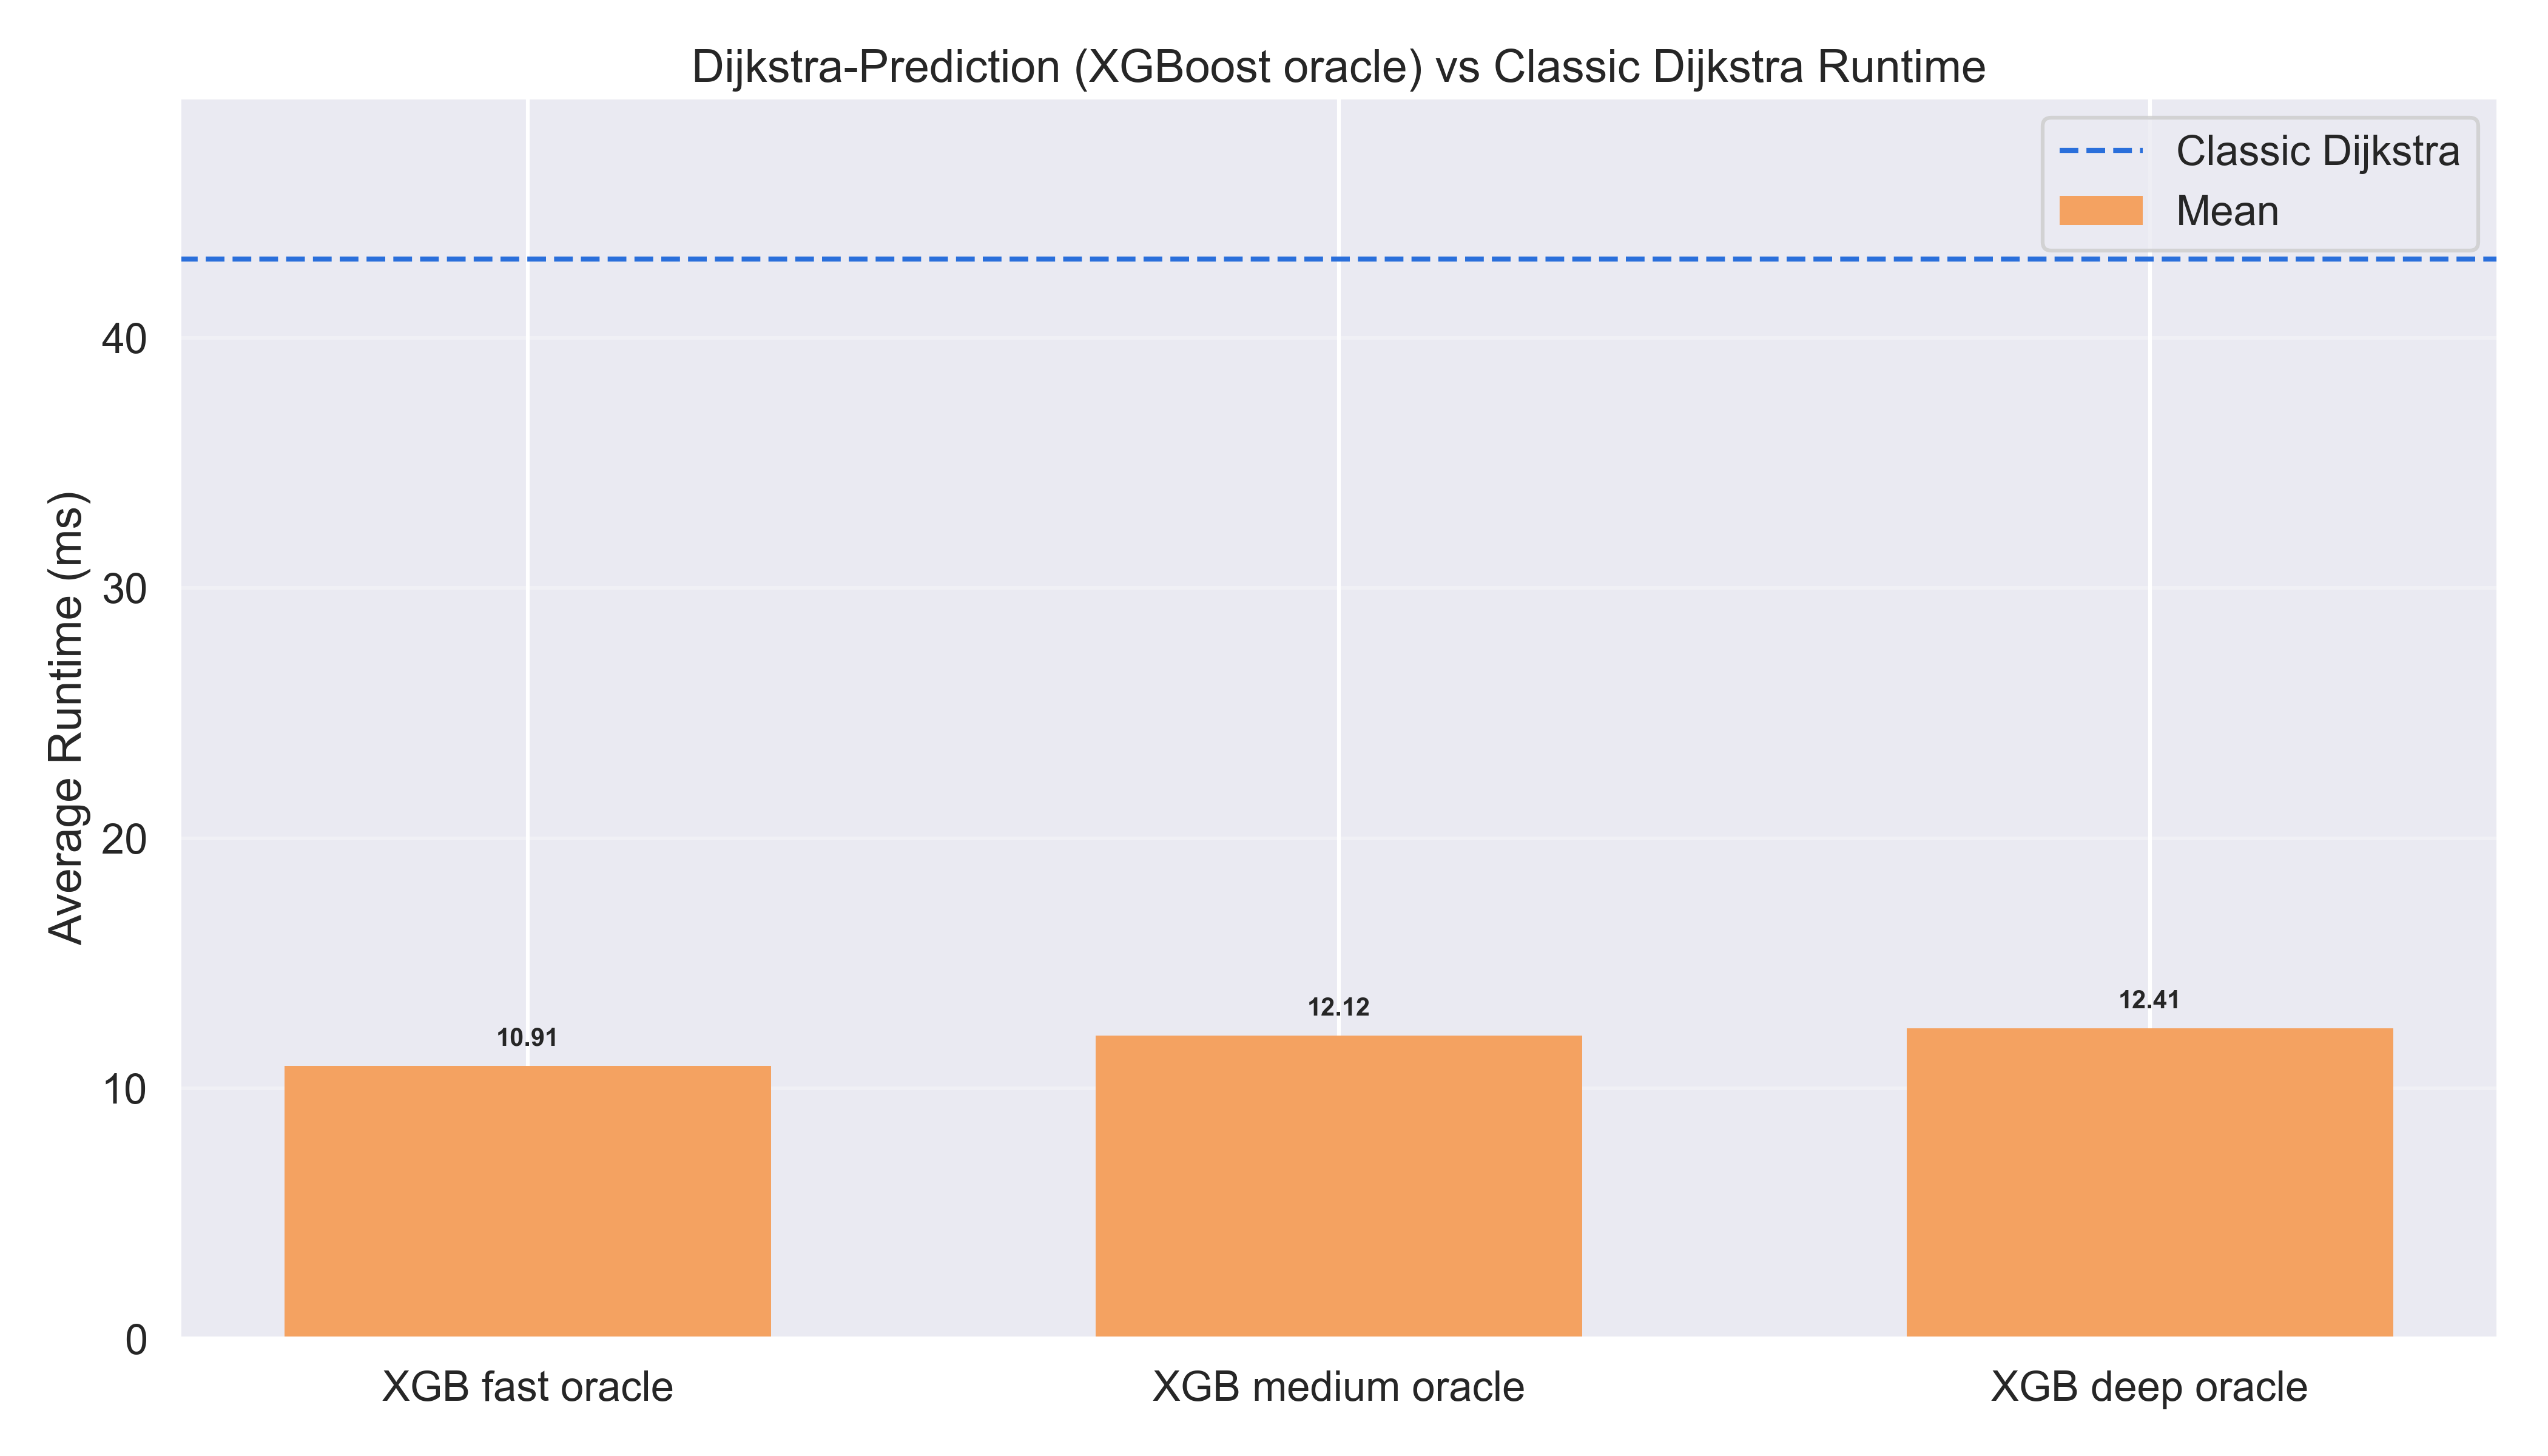
\includegraphics[width=1\linewidth]{tex/images/xgb_time_comparison.png}
    \caption{Average execution runtime (ms) for the XGBoost variants versus the classic approach.}
    \label{fig:xgboost_runtime}
\end{figure}

\begin{table}[h]
\centering
\caption{Average Runtime (ms) with XGBoost oracle architectures.}
\label{tab:xgboost_runtime}
\renewcommand{\tabularxcolumn}[1]{m{#1}}
\begin{tabularx}{\textwidth}{
    >{\centering\arraybackslash}X 
    >{\centering\arraybackslash}X 
}
\toprule
\textbf{Oracle Model Architecture} & \textbf{Average Runtime per Graph (ms)} \\ \midrule
XGBoost Deep (300,5,0.05)  & 12.41 \\
XGBoost Medium (200,4,0.05) & 12.11 \\
XGBoost Fast (100,3,0.1)  & 10.90 \\ \midrule
\texttt{DIJKSTRA} & 43.15 \\ \bottomrule
\end{tabularx}
\end{table}

The \texttt{DIJKSTRA-PREDICTION} algorithm utilizing XGBoost achieved average execution times ranging from $10.90$ms to $12.41$ms. This represents a massive reduction compared to the $43.15$ms baseline of the classic algorithm, a reduction of $\approx72\%$. Notably, the \texttt{Fast} variant has the fastest execution time, reflecting on it's smaller amount of depth and estimators. However, as established in the prior section, fluctuations of such a small scale can be caused by system-level, hardware, interpreter or background issues, and therefore cannot definitively be attributed to the architecture's lower complexity.

\subsection{Overall Algorithmic Acceleration}
\label{subsec:overall_acceleration}

Having presented multiple experiments of the algorithm utilizing many different oracle architectures, to finalize our evaluations, we present a direct comparison of \texttt{DIJKSTRA-PREDICTION} with the MLP(16x16) oracle against the classic \texttt{DIJKSTRA} algorithm, to align with the foundational architecture proposed by Feijen and Schäfer.

As depicted in Tables \ref{tab:final_prio}, \ref{tab:final_runtime} and Figures \ref{fig:final_ops_comparison}, \ref{fig:final_runtime_comparison}, the \textsc{DIJKSTRA-PREDICTION} algorithm Feijen and Schäfer proposed is highly effective. By pruning the search space, the average Priority Queue operations are slashed from an average of $382.7$ per graph to an average of $139.4$ per graph (a $63.57\%$ reduction). This reduction in operations leads to a reduction in the execution time from an average of $43.15$ms to just $10.63$ms (a $75.36\%$ acceleration), proving that the computational time saved by skipping nodes outweighs the cost to infer the neural network at step $i_0$.
\vspace{1cm}

\begin{table}[h]
\centering
\caption{Average Priority Queue Difference.}
\label{tab:final_prio}
\renewcommand{\tabularxcolumn}[1]{m{#1}}
\begin{tabularx}{\textwidth}{
    >{\centering\arraybackslash}X 
    >{\centering\arraybackslash}X 
    >{\centering\arraybackslash}X 
}
\toprule
\textbf{Algorithm} & \textbf{Average Priority Queue Operations} & \textbf{Percentage Difference} \\ \midrule
\texttt{DIJKSTRA} & 382.7 & \textit{baseline} \\ 
\texttt{DIJKSTRA-PREDICTION}  & 139.4 & -63.57\% \\\bottomrule
\end{tabularx}
\end{table}

\begin{table}[p] % Το [p] αναγκάζει όλο το block να κάτσει σε μια αποκλειστική σελίδα για floats
\centering

% 1. Ο Πίνακας στην κορυφή
\caption{Average Runtime Difference (ms).}
\label{tab:final_runtime}
\renewcommand{\tabularxcolumn}[1]{m{#1}}
\begin{tabularx}{\textwidth}{
    >{\centering\arraybackslash}X 
    >{\centering\arraybackslash}X 
    >{\centering\arraybackslash}X 
}
\toprule
\textbf{Algorithm} & \textbf{Average Runtime (ms)} & \textbf{Percentage Speedup} \\ \midrule
\texttt{DIJKSTRA}            & 43.15 & \textit{Baseline} \\ 
\texttt{DIJKSTRA-PREDICTION} & 10.63 & \textbf{-75.36\%} \\ \bottomrule
\end{tabularx}

\vspace{1cm} % Μεγάλο κενό ανάμεσα στον πίνακα και την πρώτη εικόνα

% 2. Η πρώτη εικόνα (Operations)
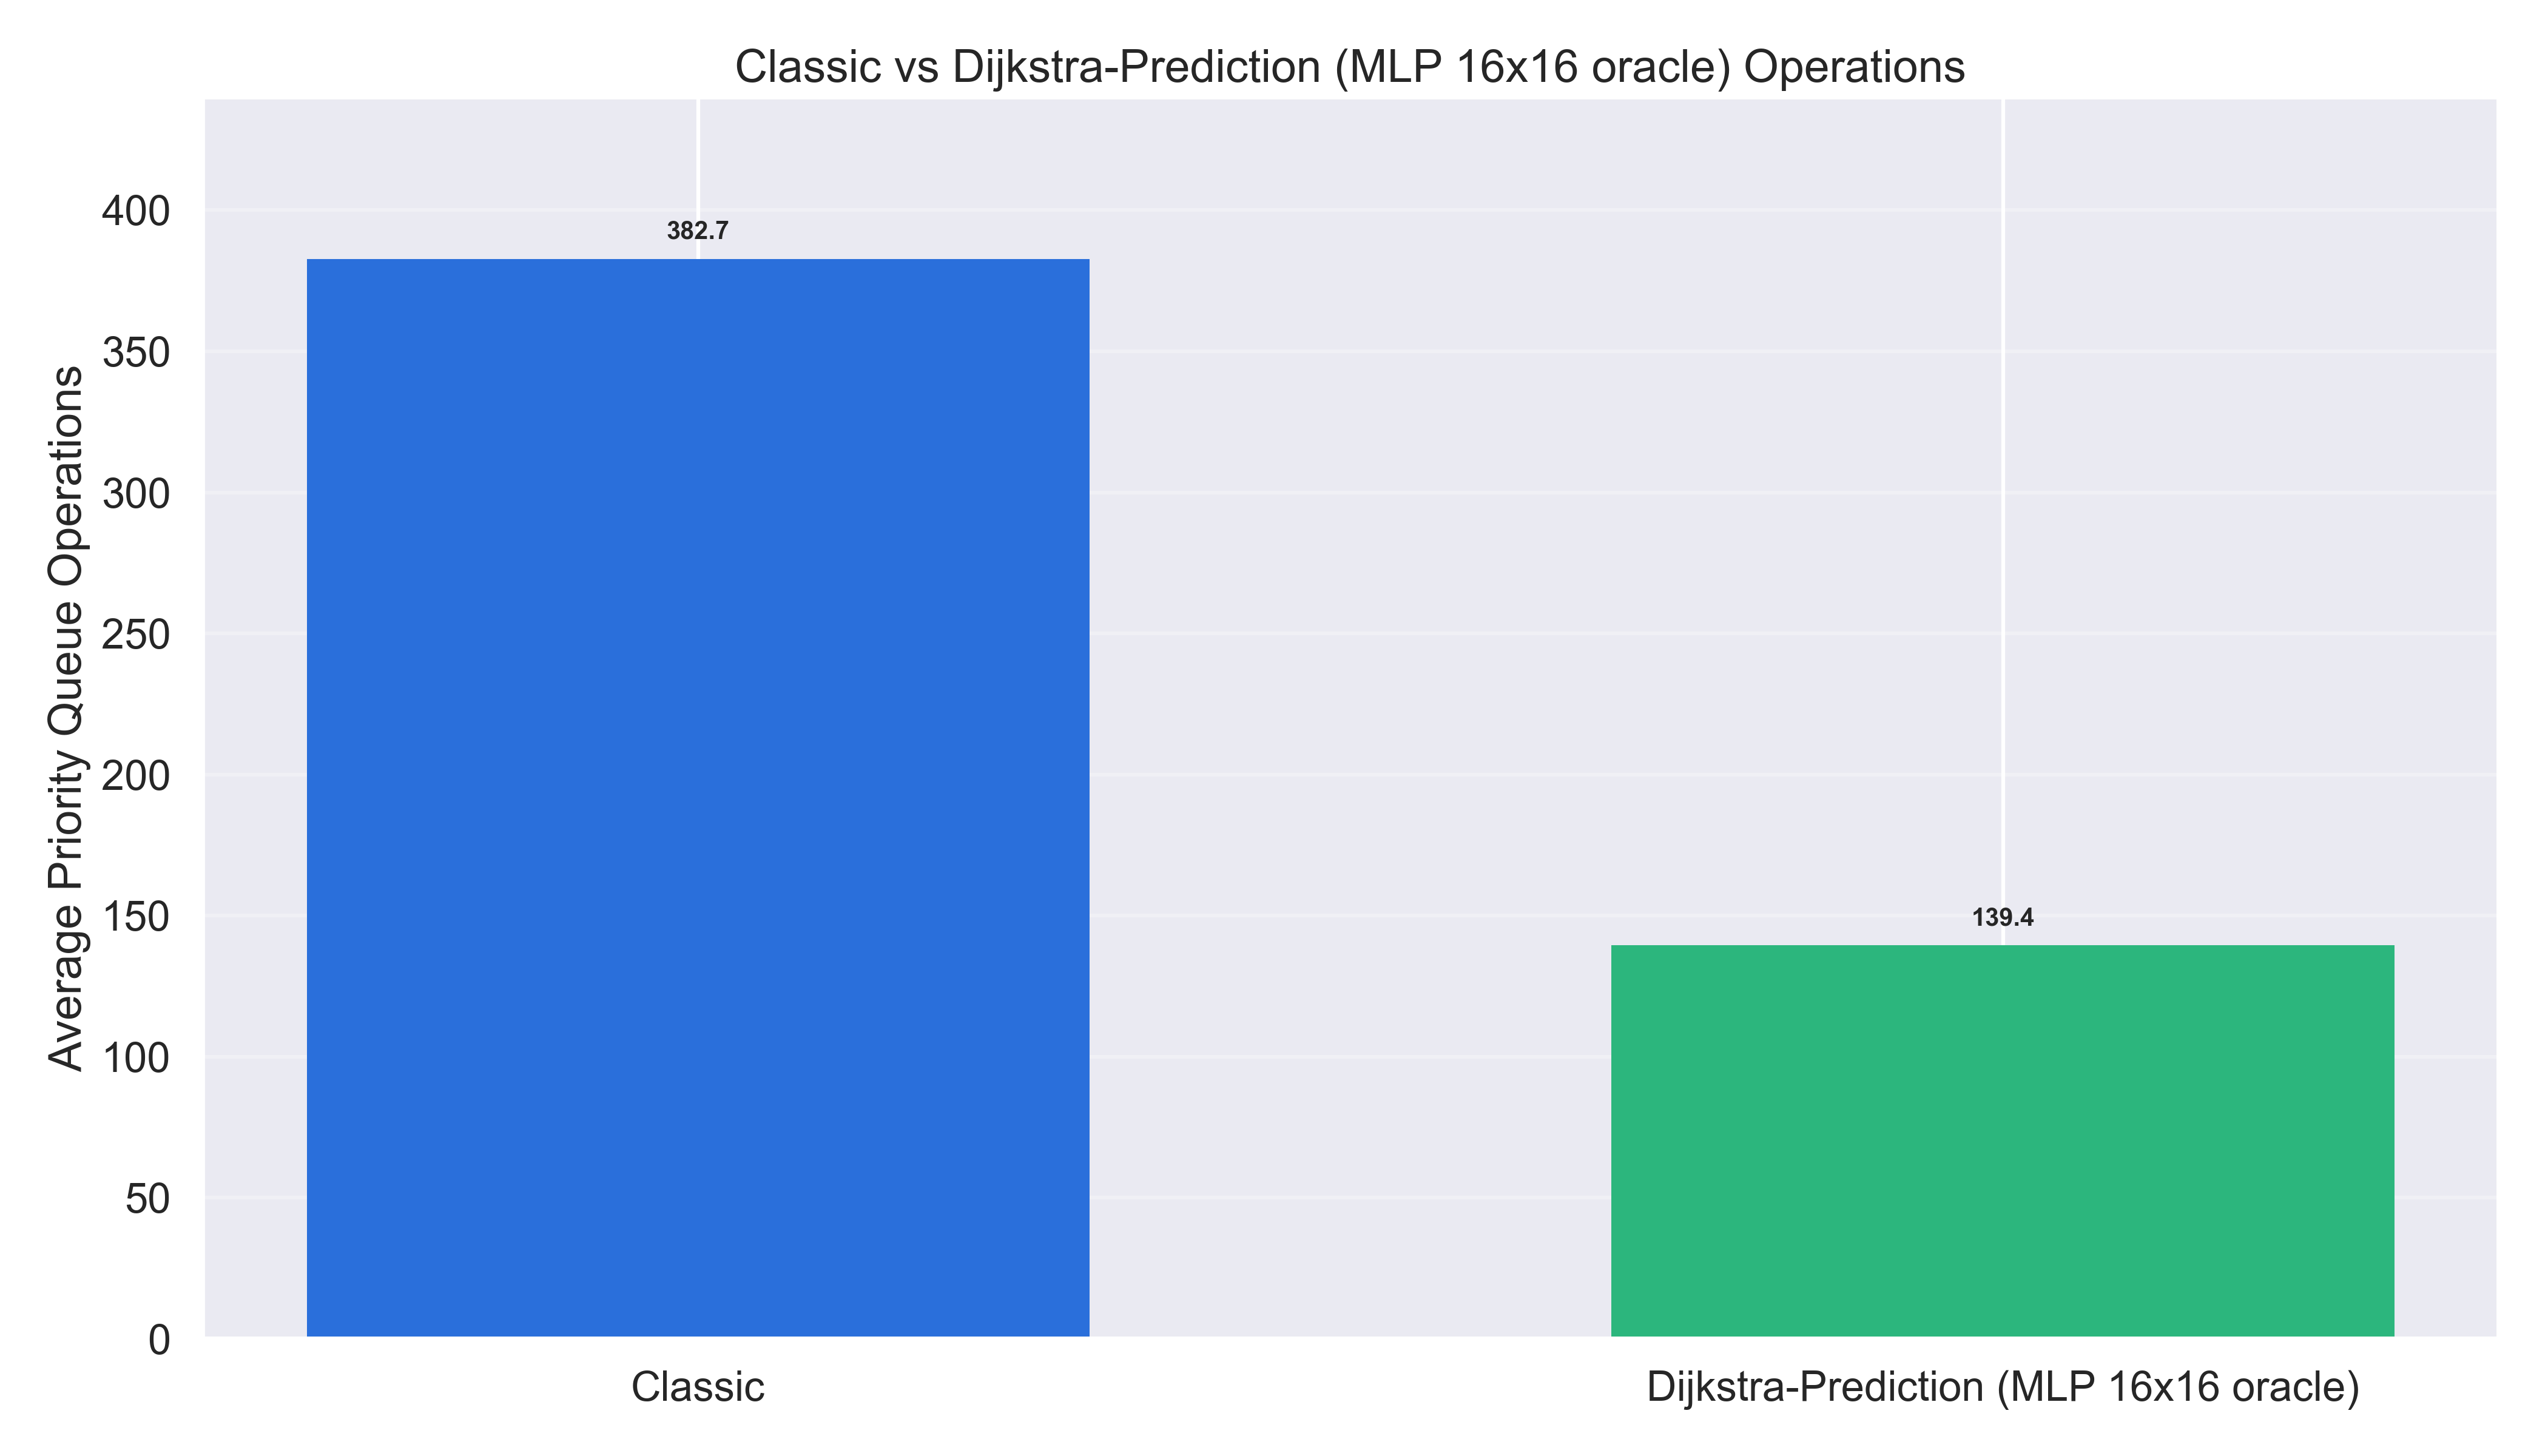
\includegraphics[width=0.8\linewidth]{tex/images/classic_vs_mlp16_ops.png}
\makeatletter\def\@captype{figure}\makeatother % "Ξεγελάει" το LaTeX για να βάλει σωστό Caption εικόνας μέσα σε περιβάλλον Table
\caption{Direct comparison of average Priority Queue operations.}
\label{fig:final_ops_comparison}

\vspace{1.0cm} % Κενό ανάμεσα στις δύο εικόνες

% 3. Η δεύτερη εικόνα (Runtime)
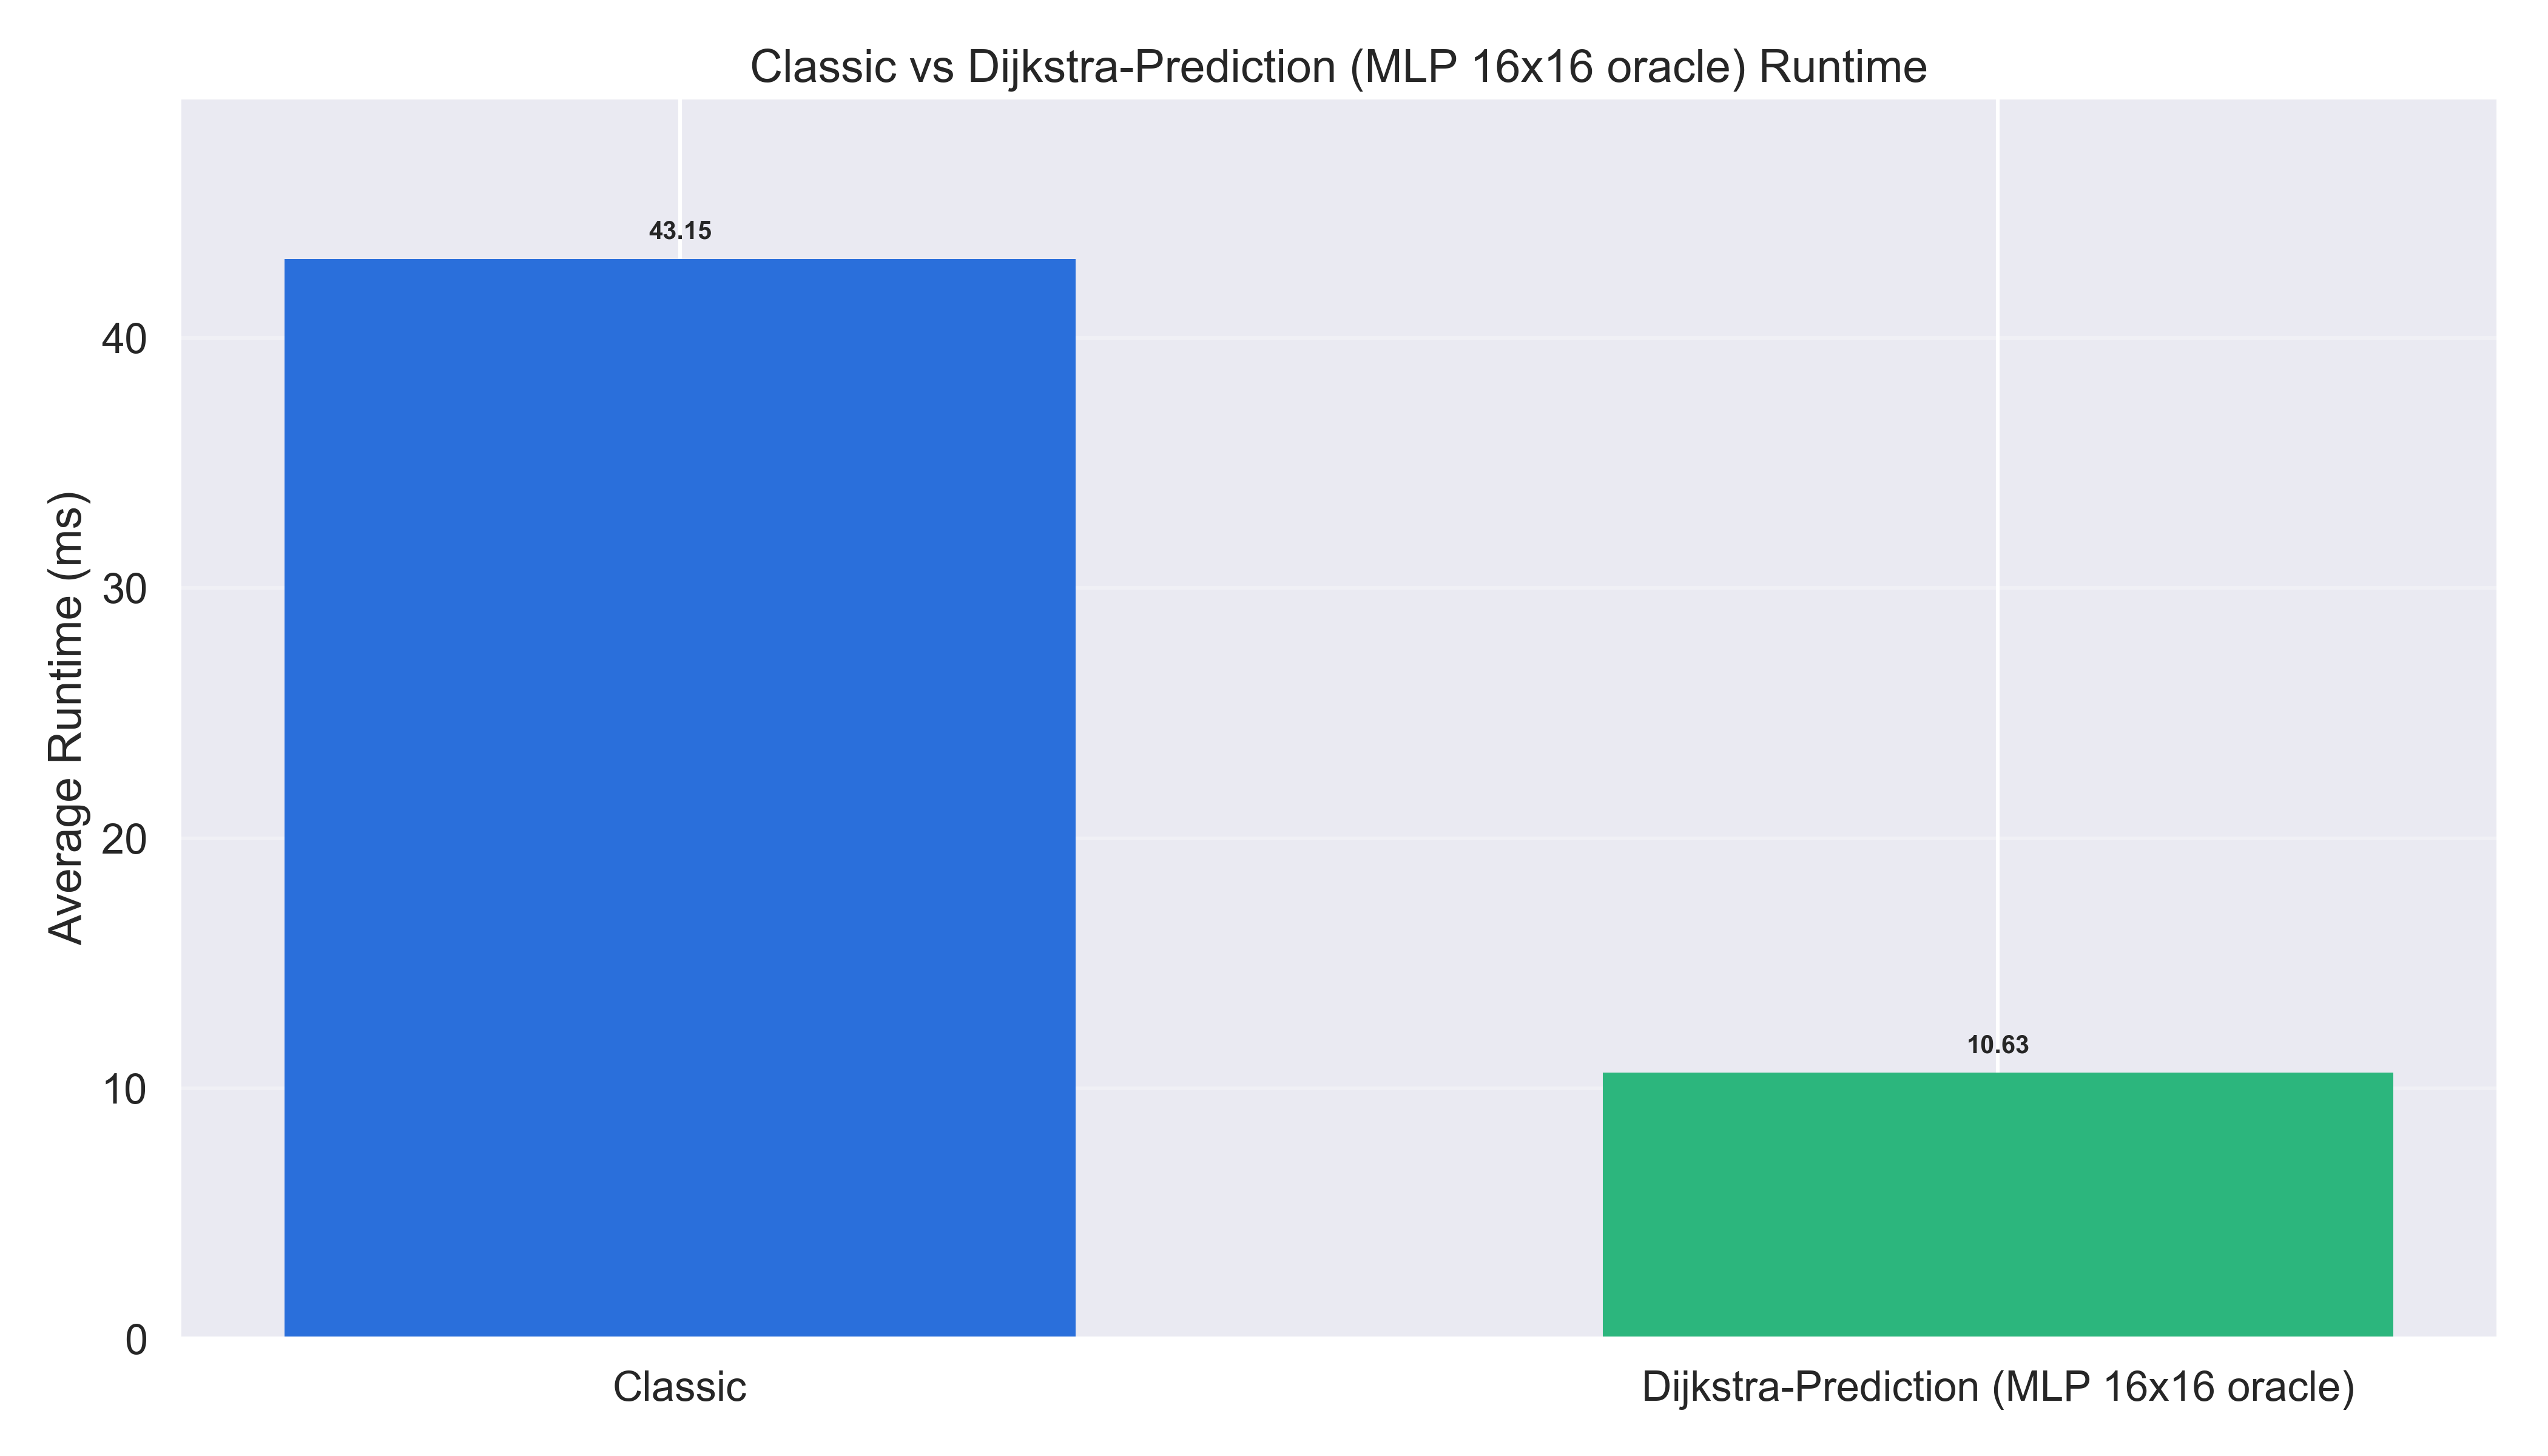
\includegraphics[width=0.8\linewidth]{tex/images/classic_vs_mlp16_time.png}
\makeatletter\def\@captype{figure}\makeatother
\caption{Direct comparison of average execution runtime (ms).}
\label{fig:final_runtime_comparison}

\end{table}

\newpage

The macroscopic impact of this optimization is best visualized in Figure \ref{fig:final_cumulative_ops}, which tracks the cumulative Priority Queue operations over the entire evaluation. The divergence between the two execution paths is continuously expanding which further highlights the achievement of the learning-augmented approach. Over 10,000 graphs, the classic algorithm wastes a large amount of operations exploring irrelevant topologies. In contrast, the ML approach restricts the boundary expansion through its prediction value $P$, leading to a faster execution.

\begin{figure}[h]
    \centering
    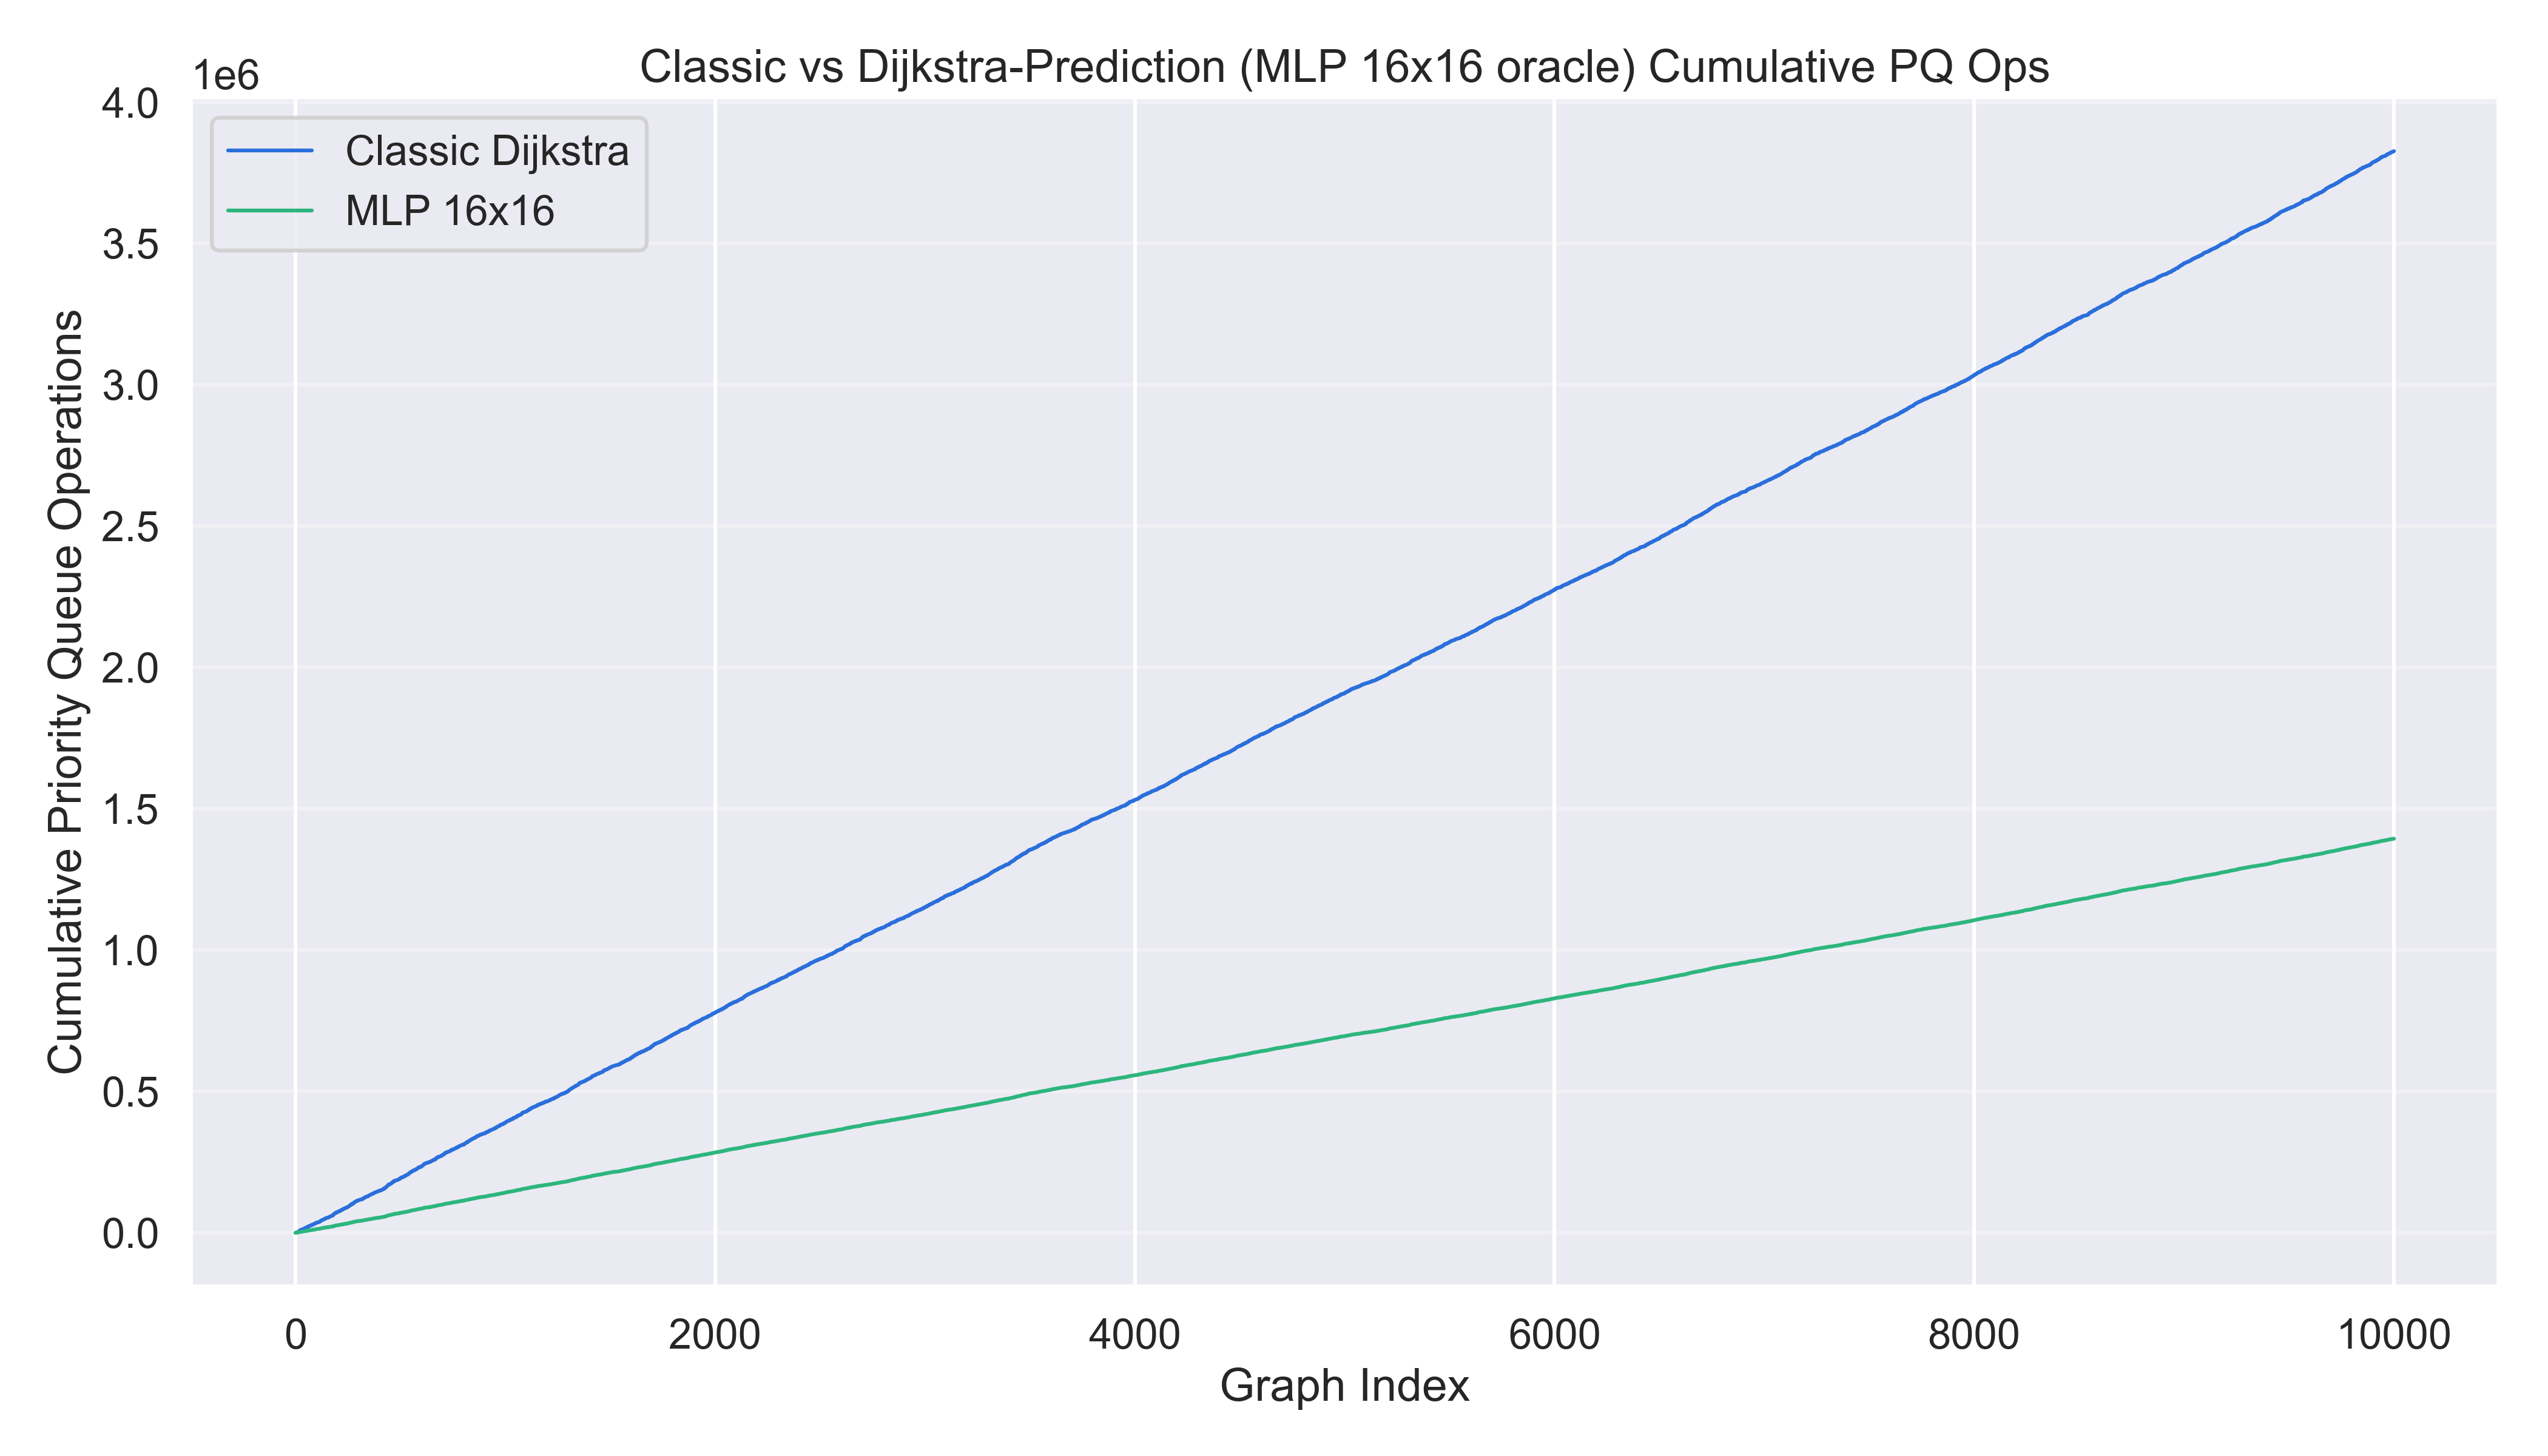
\includegraphics[width=1\linewidth]{tex/images/classic_vs_mlp16_ops_cum_line.png}
    \caption{Cumulative Priority Queue operations over the 10,000-graph dataset.}
    \label{fig:final_cumulative_ops}
\end{figure}